\section{Universal Transformer for Sequence Modeling}
\todo{add stuff}
In this section, we address the following research question:
\resq{c6.2}
We evaluate Universal Transformers on a range of algorithmic and language understanding tasks and discuss the results.

\subsection{bAbI Question-Answering}
The bAbi question answering dataset~\citep{weston2015towards} consists of 20 different synthetic tasks\footnote{\url{https://research.fb.com/downloads/babi}}. The aim is that each task tests a unique aspect of language understanding and reasoning, including the ability of: reasoning from supporting facts in a story, answering true/false type questions, counting, understanding negation and indefinite knowledge, understanding coreferences, time reasoning, positional and size reasoning, path-finding, and understanding motivations (to see examples for each of these tasks, please refer to Table 1 in \citep{weston2015towards}).

There are two versions of the dataset, one with 1k training examples and the other with 10k examples. It is important for a model to be data-efficient to achieve good results using only the 1k training examples. Moreover, the original idea is that a single model should be evaluated across all the tasks (not tuning per task), which is the \emph{train joint} setup in Tables~\ref{tab:babi-results} and ~\ref{tbl:babi_details}.

A standard Transformer does not achieve good results on this task\footnote{We experimented with different hyper-parameters and different network sizes, but it always overfits.}. However, we have designed a model based on the Universal Transformer which achieves state-of-the-art results on this task.

To encode the input, similar to~\cite{henaff2016tracking}, we first encode each fact in the story by applying a learned multiplicative positional mask to each word's embedding, and summing up all embeddings.
We embed the question in the same way, and then feed the (Universal) Transformer with these embeddings of the facts and questions. 

As originally proposed, models can either be trained on each task separately (``train single'') or jointly on all tasks (``train joint''). Table~\ref{tab:babi-results} summarizes our results. We conducted 10 runs with different initializations and picked the best model based on performance on the validation set, similar to previous work. Both the UT and UT with dynamic halting achieve state-of-the-art results on all tasks in terms of average error and number of failed tasks\footnote{Defined as $> 5\%$ error.}, in both the 10K and 1K training regime. Tables~\ref{tbl:babi_details} presents the results of best and average results of 10 runs breakdown by task.

\begin{table}[t!]
\centering
\begin{adjustbox}{max width=\textwidth}
\begin{tabular}{lllll}
& & & & \\ \toprule
\multirow{2}{*}{ \bf Model } & \multicolumn{2}{c}{ \bf 10K examples } & \multicolumn{2}{c}{ \bf 1K examples } \\ \cmidrule{2-5}
& train single & train joint & train single & train joint \\ \midrule
\multicolumn{5}{c}{\bf Previous best results:} \\ \midrule
QRNet~\citep{seo2016query} & 0.3 (0/20) & - & - & - \\
Sparse DNC~\citep{rae2016scaling} & - & 2.9 (1/20) & - & - \\
GA+MAGE~\cite{dhingra2017linguistic} & - & - & 8.7 (5/20) & - \\
MemN2N~\cite{sukhbaatar2015} & - & - & -  & 12.4 (11/20) \\\midrule
\multicolumn{5}{c}{\bf Our Results:} \\ \midrule
Transformer~\citep{transformer} & 15.2 (10/20) & 22.1 (12/20) & 21.8 (5/20) & 26.8 (14/20) \\
Universal Transformer (this work) & 0.23 (0/20) & 0.47 (0/20) & 5.31 (5/20) & 8.50 (8/20) \\
UT w/ dynamic halting (this work) & {\bf 0.21 (0/20)} & {\bf 0.29 (0/20)} & {\bf 4.55 (3/20)} & {\bf 7.78 (5/20)} \\ \bottomrule
\end{tabular}
\end{adjustbox}
\caption{Average error and number of failed tasks ($> 5\%$ error) out of 20 (in parentheses; lower is better in both cases) on the bAbI dataset under the different training/evaluation setups. We indicate state-of-the-art where available for each, or `-' otherwise.}
\label{tab:babi-results}
\end{table}
\begin{table}[t!]
\centering
\caption{Detailed results on the bAbI question answering tasks.}
\label{tbl:babi_details}
\begin{subtable}{0.6\textwidth}
\centering
\begin{adjustbox}{max width=\textwidth}
\begin{tabular}{lcccc}
\toprule
\multicolumn{5}{c}{Best seed run for each task (out of 10 runs) } \\ \midrule
\multirow{2}{*}{ Task id } & \multicolumn{2}{c}{ 10K } & \multicolumn{2}{c}{ 1K } \\  \cmidrule{2-5}
& train single & train joint & train single & train joint \\ \midrule
1 & 0.0 & 0.0 & 0.0 & 0.0 \\
2 & 0.0 & 0.0 & 0.0 & 0.5 \\
3 & 0.4 & 1.2 & 3.7 & 5.4 \\
4 & 0.0 & 0.0 & 0.0 & 0.0 \\
5 & 0.0 & 0.0 & 0.0 & 0.5 \\
6 & 0.0 & 0.0 & 0.0 & 0.5 \\
7 & 0.0 & 0.0 & 0.0 & 3.2 \\
8 & 0.0 & 0.0 & 0.0 & 1.6 \\
9 & 0.0 & 0.0 & 0.0 & 0.2 \\
10 & 0.0 & 0.0 & 0.0 & 0.4 \\
11 & 0.0 & 0.0 & 0.0 & 0.1 \\
12 & 0.0 & 0.0 & 0.0 & 0.0 \\
13 & 0.0 & 0.0 & 0.0 & 0.6 \\
14 & 0.0 & 0.0 & 0.0 & 3.8 \\
15 & 0.0 & 0.0 & 0.0 & 5.9 \\
16 & 0.4 & 1.2 & 5.8 & 15.4 \\
17 & 0.6 & 0.2 & 32.0 & 42.9 \\
18 & 0.0 & 0.0 & 0.0 & 4.1 \\
19 & 2.8 & 3.1 & 47.1 & 68.2 \\
20 & 0.0 & 0.0 & 2.4 & 2.4 \\ \midrule
avg err & 0.21 & 0.29 & 4.55 & 7.78 \\ \midrule
failed & 0 & 0 & 3 & 5 \\
\bottomrule
\end{tabular}
\end{adjustbox}
\end{subtable}
\\
\vspace{10pt}
\begin{subtable}{0.6\textwidth}
\centering
\begin{adjustbox}{max width=\textwidth}
\begin{tabular}{lcccc}
\toprule
\multicolumn{5}{c}{Average (\rpm var) over all seeds (for 10 runs)} \\ \midrule
\multirow{2}{*}{ Task id } & \multicolumn{2}{c}{ 10K } & \multicolumn{2}{c}{ 1K } \\  \cmidrule{2-5}
& train single & train joint & train single & train joint \\ \midrule
1 & 0.0 \rpm 0.0 & 0.0 \rpm 0.0 & 0.2 \rpm 0.3 & 0.1 \rpm 0.2 \\ 
2 & 0.2 \rpm 0.4 & 1.7 \rpm 2.6 & 3.2 \rpm 4.1 & 4.3 \rpm 11.6 \\ 
3 & 1.8 \rpm 1.8 & 4.6 \rpm 7.3 & 9.1 \rpm 12.7 & 14.3 \rpm 18.1 \\ 
4 & 0.1 \rpm 0.1 & 0.2 \rpm 0.1 & 0.3 \rpm 0.3 & 0.4 \rpm 0.6 \\ 
5 & 0.2 \rpm 0.3 & 0.8 \rpm 0.5 & 1.1 \rpm 1.3 & 4.3 \rpm 5.6 \\ 
6 & 0.1 \rpm 0.2 & 0.1 \rpm 0.2 & 1.2 \rpm 2.1 & 0.8 \rpm 0.4 \\ 
7 & 0.3 \rpm 0.5 & 1.1 \rpm 1.5 & 0.0 \rpm 0.0 & 4.1 \rpm 2.9 \\ 
8 & 0.3 \rpm 0.2 & 0.5 \rpm 1.1 & 0.1 \rpm 0.2 & 3.9 \rpm 4.2 \\ 
9 & 0.0 \rpm 0.0 & 0.0 \rpm 0.0 & 0.1 \rpm 0.1 & 0.3 \rpm 0.3 \\ 
10 & 0.1 \rpm 0.2 & 0.5 \rpm 0.4 & 0.7 \rpm 0.8 & 1.3 \rpm 1.6 \\ 
11 & 0.0 \rpm 0.0 & 0.1 \rpm 0.1 & 0.4 \rpm 0.8 & 0.3 \rpm 0.9 \\ 
12 & 0.2 \rpm 0.1 & 0.4 \rpm 0.4 & 0.6 \rpm 0.9 & 0.3 \rpm 0.4 \\ 
13 & 0.2 \rpm 0.5 & 0.3 \rpm 0.4 & 0.8 \rpm 0.9 & 1.1 \rpm 0.9 \\ 
14 & 1.8 \rpm 2.6 & 1.3 \rpm 1.6 & 0.1 \rpm 0.2 & 4.7 \rpm 5.2 \\ 
15 & 2.1 \rpm 3.4 & 1.6 \rpm 2.8 & 0.3 \rpm 0.5 & 10.3 \rpm 8.6 \\ 
16 & 1.9 \rpm 2.2 & 0.9 \rpm 1.3 & 9.1 \rpm 8.1 & 34.1 \rpm 22.8 \\ 
17 & 1.6 \rpm 0.8 & 1.4 \rpm 3.4 & 43.7 \rpm 18.6 & 51.1 \rpm 12.9 \\ 
18 & 0.3 \rpm 0.4 & 0.7 \rpm 1.4 & 2.3 \rpm 3.6 & 12.8 \rpm 9.0 \\ 
19 & 3.4 \rpm 4.0 & 6.1 \rpm 7.3 & 50.2 \rpm 8.4 & 73.1 \rpm 23.9 \\ 
20 & 0.0 \rpm 0.0 & 0.0 \rpm 0.0 & 3.2 \rpm 2.5 & 2.6 \rpm 2.8 \\ \midrule
avg & 0.73 \rpm 0.89 & 1.12 \rpm 1.62 & 6.34 \rpm 3.32 & 11.21 \rpm 6.65 \\ 
\bottomrule
\end{tabular}
\end{adjustbox}
\end{subtable}
\end{table}
\afterpage{\clearpage}


To understand the working of the model better, we analyzed both the attention distributions and the average ACT ponder times for this task. First, we observe that the attention distributions start out very uniform, but get progressively sharper in later steps around the correct supporting facts that are required to answer each question, which is indeed very similar to how humans would solve the task. 
%
Second, with dynamic halting we observe that the average ponder time (i.e.\ depth of the per-symbol recurrent processing chain) over all positions in all samples in the test data for tasks requiring three supporting facts is higher ($3.8 \rpm 2.2$) than for tasks requiring only two ($3.1 \rpm 1.1$), which is in turn higher than for tasks requiring only one supporting fact ($2.3 \rpm 0.8$). This indicates that the model adjusts the number of processing steps with the number of supporting facts required to answer the questions. 

\begin{figure}[t]
 \centering
 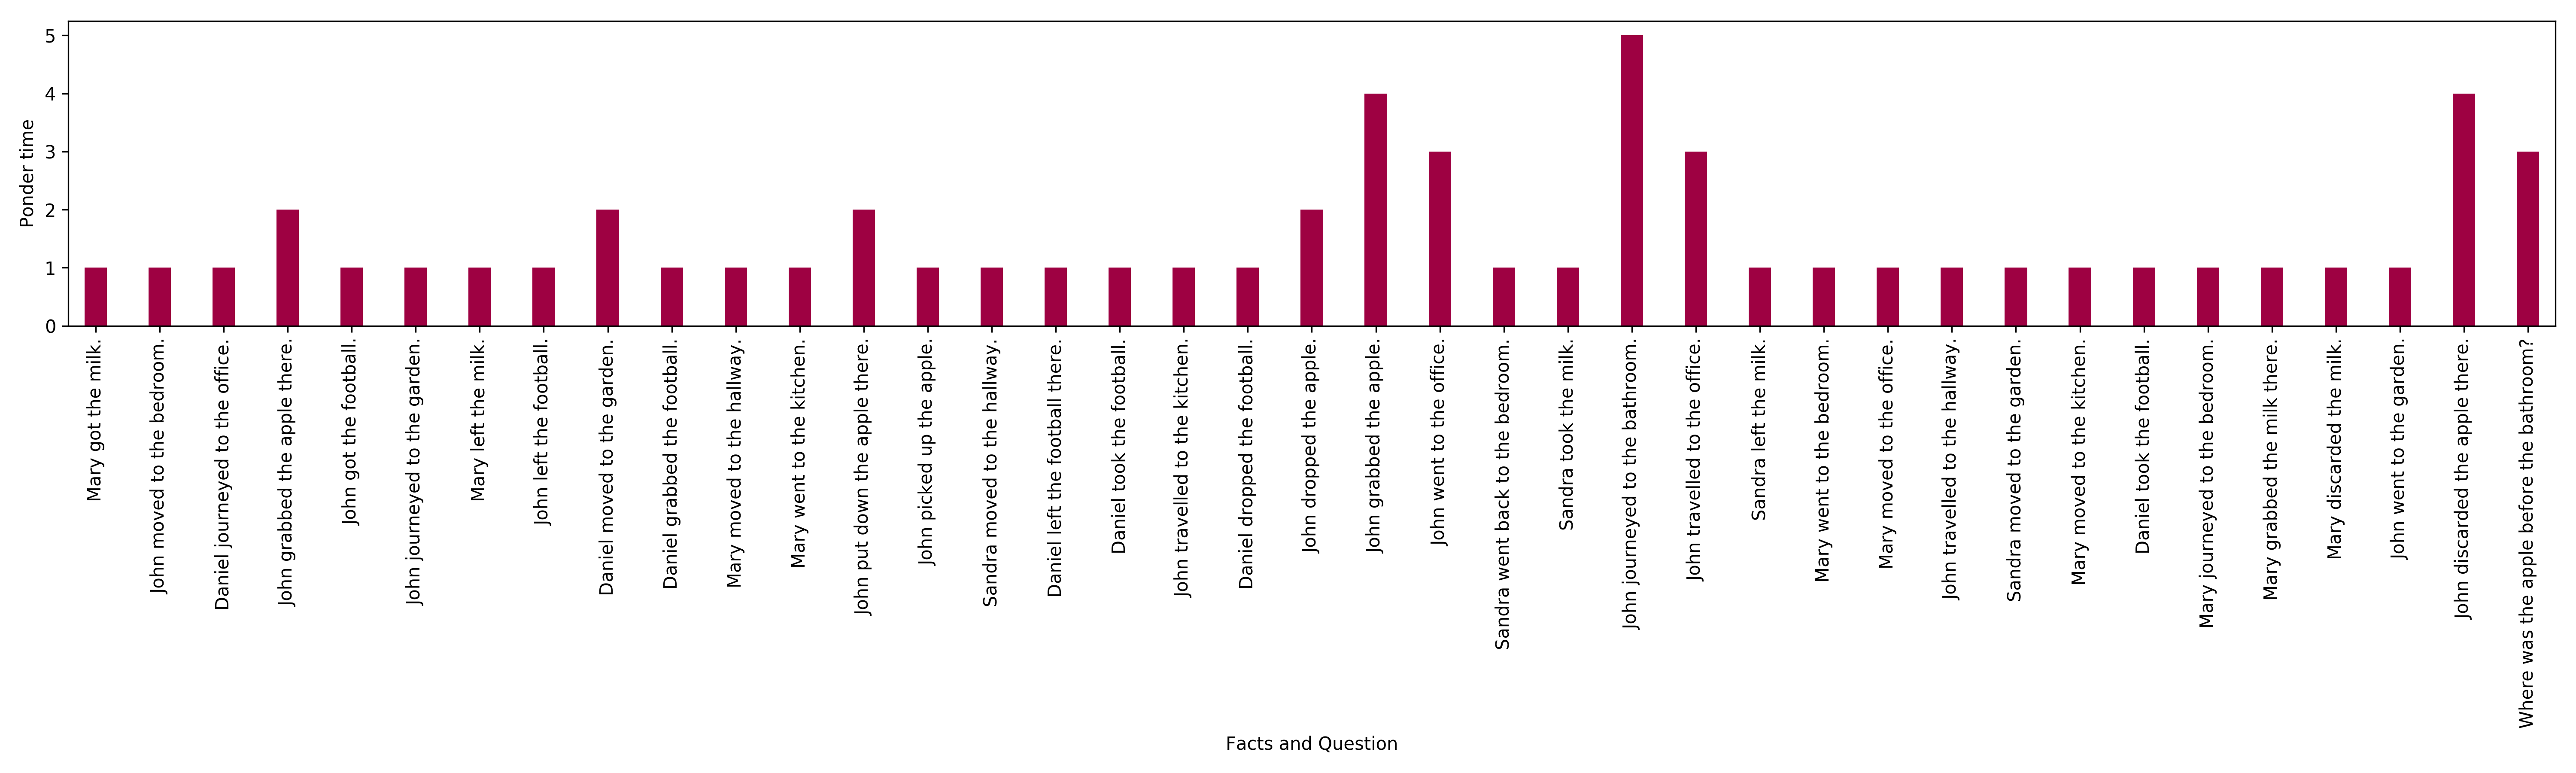
\includegraphics[width=\textwidth]{04-part-03/chapter-06/figs_and_tables/fig_task3_example_ponder.png}
 \caption{Ponder time of UT with dynamic halting for encoding facts in a story and question in a bAbI task requiring three supporting facts.}
 \label{fig:act_ponder}
\end{figure}
Finally, we observe that the histogram of ponder times at different positions is more uniform in tasks requiring only one supporting fact compared to two and three, and likewise for tasks requiring two compared to three.  Especially for tasks requiring three supporting facts, many positions halt at step 1 or 2 already and only a few get transformed for more steps (see for example Figure~\ref{fig:act_ponder}). This is particularly interesting as the length of stories is indeed much higher in this setting, with more irrelevant facts which the model seems to successfully learn to ignore in this way.

Similar to dynamic memory networks~\citep{kumar2016ask}, there is an iterative attention process in UTs that allows the model to condition its attention over memory on the result of previous iterations. 
%

\begin{figure}[!ht]
\begin{minipage}{\textwidth}
\fontsize{8}{8}\fontfamily{pcr}\selectfont
\begin{tabular}{l l}
\textbf{An example from tasks 1}: & \textbf{(requiring one supportive fact to solve)}\\
\\
\textbf{Story}: & \\
& John travelled to the hallway. \\
& Mary journeyed to the bathroom. \\
& Daniel went back to the bathroom. \\
& John moved to the bedroom \\
\\
\textbf{Question}: & \\
& Where is Mary? \\
\textbf{Model's output}: & \\
& bathroom
\end{tabular}
\end{minipage}
\\ \vfill
\vspace{20pt} % maximize space between the minipages
\begin{minipage}{\textwidth}
    \centering
    \begin{subfigure}[t]{\textwidth}
        \centering
        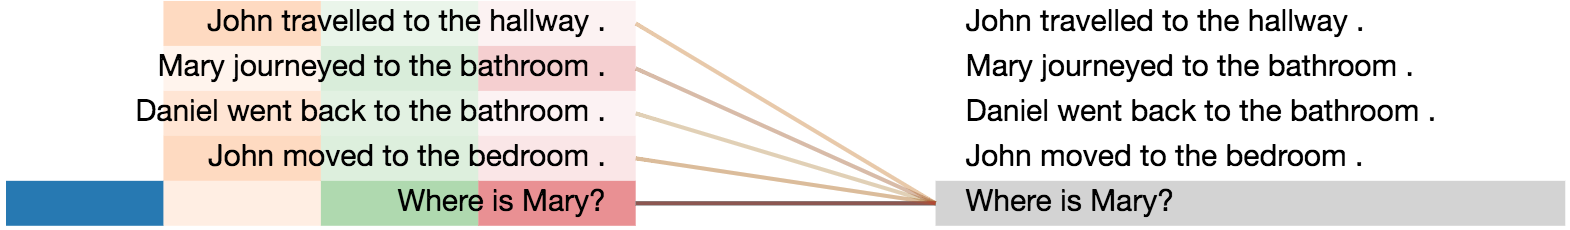
\includegraphics[height=0.8in]{04-part-03/chapter-06/figs_and_tables/figs_attention_babi/e1-step1.png}
        \caption{Step 1}
    \end{subfigure}%
    \hfill \hfill
    \begin{subfigure}[t]{\textwidth}
        \centering
        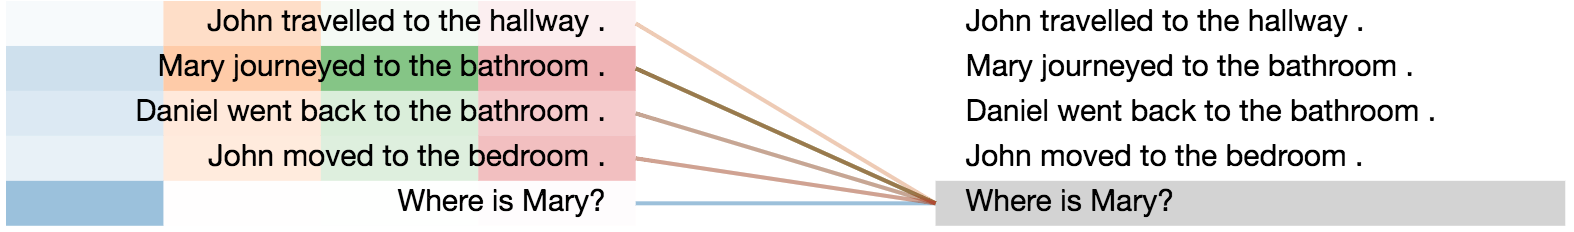
\includegraphics[height=0.8in]{04-part-03/chapter-06/figs_and_tables/figs_attention_babi/e1-step2}
        \caption{Step 2}
    \end{subfigure}
    \hfill \hfill
    \begin{subfigure}[t]{\textwidth}
        \centering
        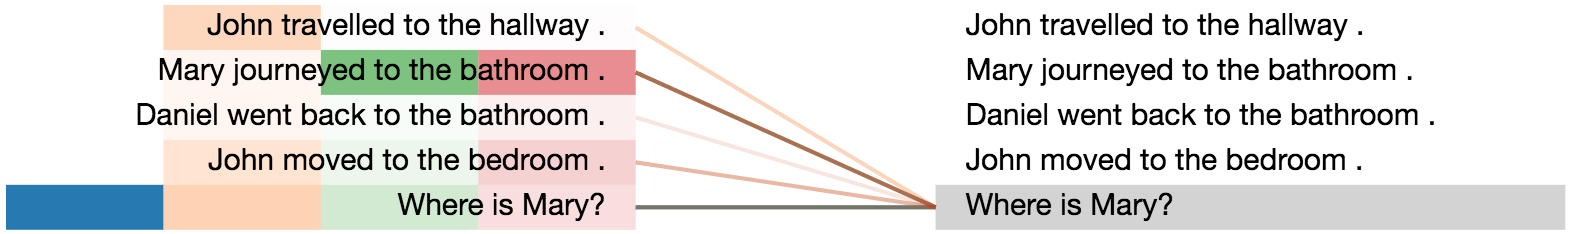
\includegraphics[height=0.8in]{04-part-03/chapter-06/figs_and_tables/figs_attention_babi/e1-step3}
        \caption{Step 3}
    \end{subfigure}
    \hfill \hfill 
    \begin{subfigure}[t]{\textwidth}
        \centering
        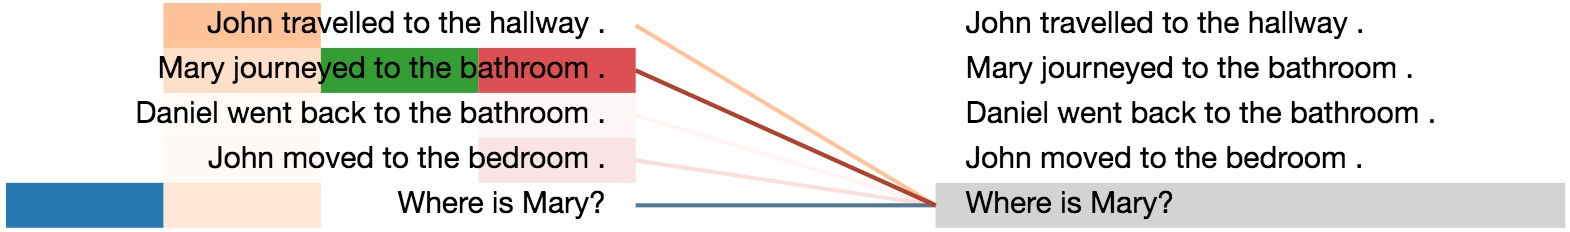
\includegraphics[height=0.8in]{04-part-03/chapter-06/figs_and_tables/figs_attention_babi/e1-step4}
        \caption{Step 4}
    \end{subfigure}
\end{minipage}
    \caption{\label{fig:ex1}Visualization of the attention distributions, when encoding the question: \emph{``Where is Mary?''}.}
\end{figure}
\afterpage{\clearpage}




\begin{figure}[!h]
\begin{minipage}{\textwidth}
\fontsize{8}{8}\fontfamily{pcr}\selectfont
\begin{tabular}{l l}
\textbf{An example from tasks 2}: & \textbf{(requiring two supportive facts to solve)}\\
\\
\textbf{Story}: & \\
& Sandra journeyed to the hallway. \\
& Mary went to the bathroom. \\
& Mary took the apple there. \\
& Mary dropped the apple. \\
\\
\textbf{Question}: & \\
& Where is the apple? \\
\textbf{Model's output}: & \\
& bathroom
\end{tabular}
\end{minipage}
\\  \vfill
\vspace{20pt} % maximize space between the minipages
\begin{minipage}{\textwidth}
    \centering
    \begin{subfigure}[t]{\textwidth}
        \centering
        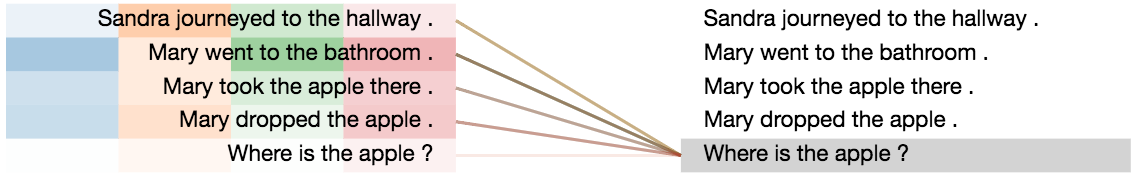
\includegraphics[height=0.8in]{04-part-03/chapter-06/figs_and_tables/figs_attention_babi/e2-step1}
        \caption{Step 1}
    \end{subfigure}%
    \hfill \hfill
    \begin{subfigure}[t]{\textwidth}
        \centering
        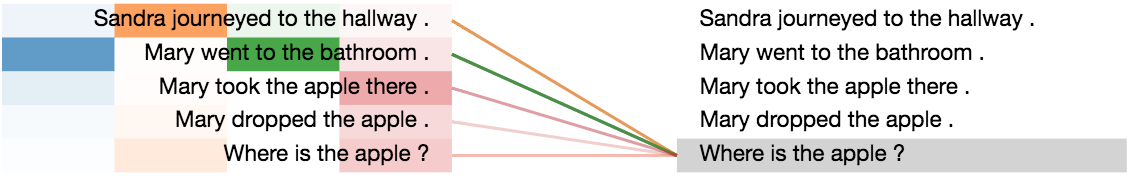
\includegraphics[height=0.8in]{04-part-03/chapter-06/figs_and_tables/figs_attention_babi/e2-step2}
        \caption{Step 2}
    \end{subfigure}
    \hfill \hfill
    \begin{subfigure}[t]{\textwidth}
        \centering
        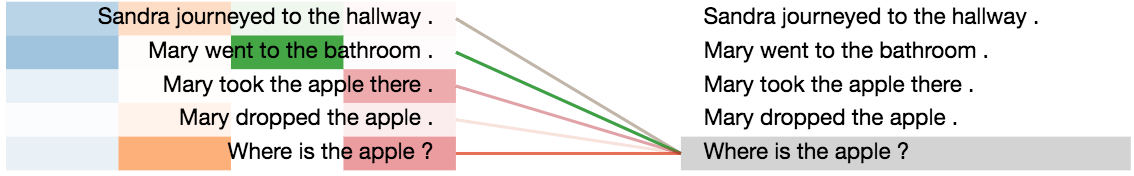
\includegraphics[height=0.8in]{04-part-03/chapter-06/figs_and_tables/figs_attention_babi/e2-step3}
        \caption{Step 3}
    \end{subfigure}
    \hfill \hfill 
    \begin{subfigure}[t]{\textwidth}
        \centering
        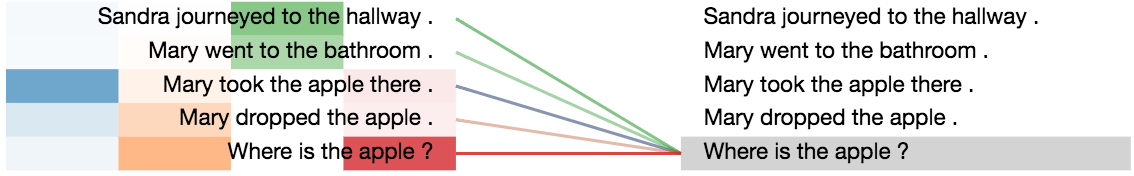
\includegraphics[height=0.8in]{04-part-03/chapter-06/figs_and_tables/figs_attention_babi/e2-step4}
        \caption{Step 4}
    \end{subfigure}
    \end{minipage}
    \caption{\label{fig:ex2}Visualization of the attention distributions, when encoding the question: \emph{``Where is the apple?''}.}
\end{figure}

\afterpage{\clearpage}

\begin{figure}[!h]
\begin{minipage}{\textwidth}
\fontsize{8}{8}\fontfamily{pcr}\selectfont
\begin{tabular}{l l}
\textbf{An example from tasks 2}: & \textbf{(requiring two supportive facts to solve)}\\
\\
\textbf{Story}: & \\
& John went to the hallway. \\
& John went back to the bathroom. \\
& John grabbed the milk there. \\
& Sandra went back to the office. \\
& Sandra journeyed to the kitchen. \\
& Sandra got the apple there. \\
& Sandra dropped the apple there. \\
& John dropped the milk. \\
\\
\textbf{Question}: & \\
& Where is the milk? \\
\textbf{Model's output}: & \\
& bathroom
\end{tabular}
\end{minipage}
\\ \vfill
\vspace{20pt} % maximize space between the minipages
\begin{minipage}{\textwidth}
    \centering
    \begin{subfigure}[t]{\textwidth}
        \centering
        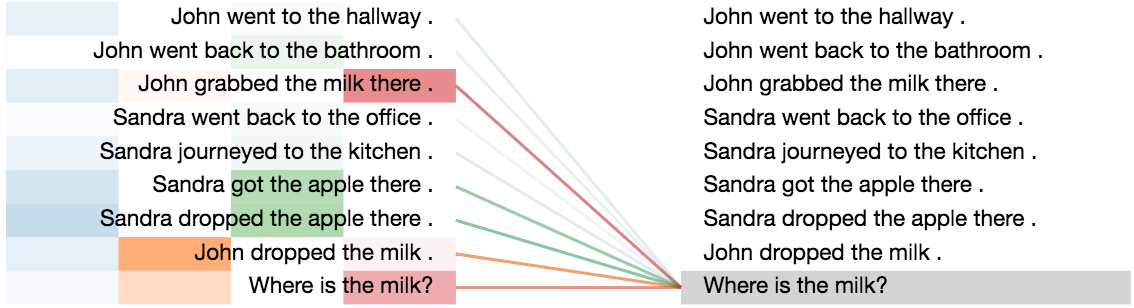
\includegraphics[height=1.3in]{04-part-03/chapter-06/figs_and_tables/figs_attention_babi/e3-step1}
        \caption{Step 1}
    \end{subfigure}%
    \hfill \hfill
    \begin{subfigure}[t]{\textwidth}
        \centering
        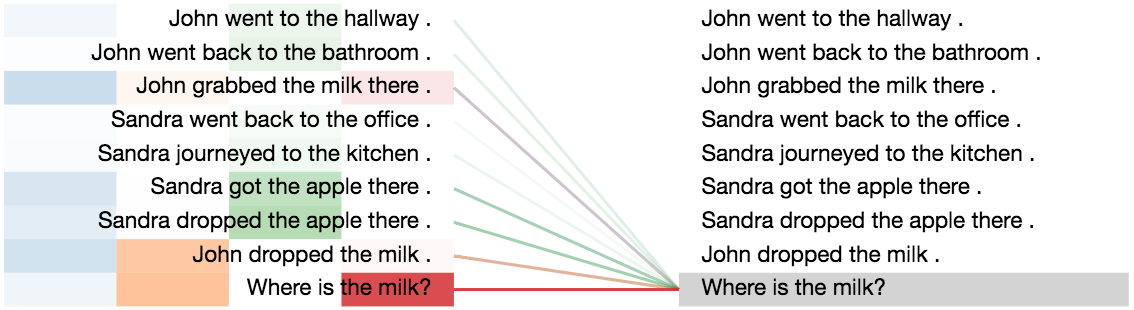
\includegraphics[height=1.3in]{04-part-03/chapter-06/figs_and_tables/figs_attention_babi/e3-step2}
        \caption{Step 2}
    \end{subfigure}
    \hfill \hfill
    \begin{subfigure}[t]{\textwidth}
        \centering
        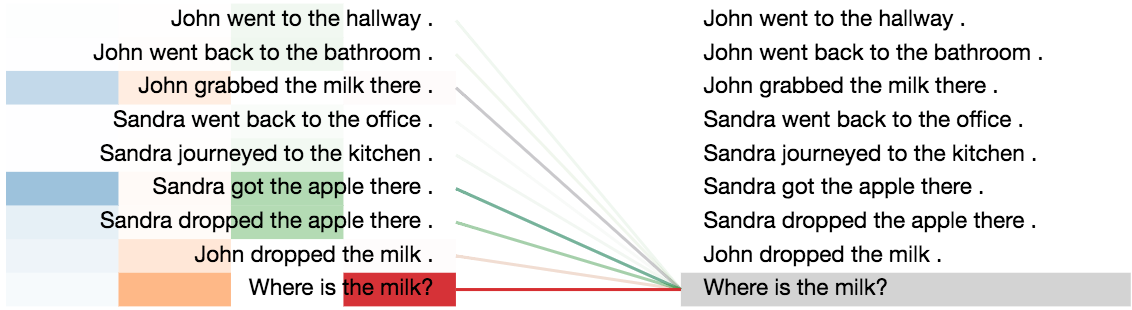
\includegraphics[height=1.3in]{04-part-03/chapter-06/figs_and_tables/figs_attention_babi/e3-step3}
        \caption{Step 3}
    \end{subfigure}
    \hfill \hfill 
    \begin{subfigure}[t]{\textwidth}
        \centering
        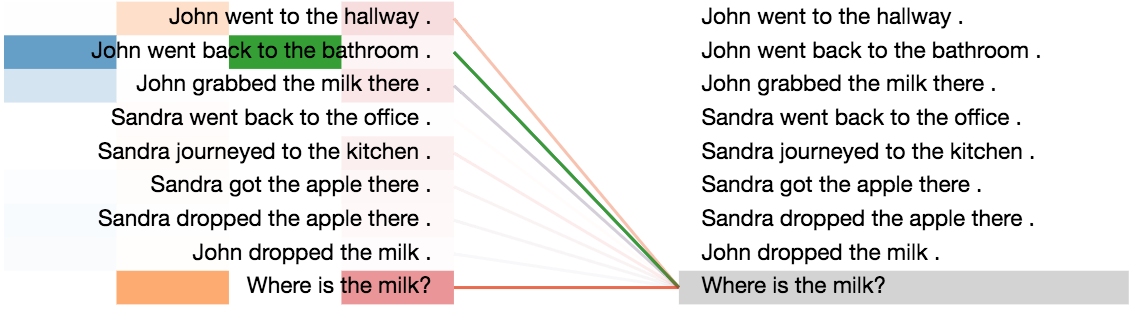
\includegraphics[height=1.3in]{04-part-03/chapter-06/figs_and_tables/figs_attention_babi/e3-step4}
        \caption{Step 4}
    \end{subfigure}
    \end{minipage}
    \caption{\label{fig:ex3}Visualization of the attention distributions, when encoding the question: \emph{``Where is the milk?''}.}
\end{figure}

\afterpage{\clearpage}

\begin{figure}[!h]
\begin{minipage}{\textwidth}
\fontsize{8}{8}\fontfamily{pcr}\selectfont
\begin{tabular}{l l}
\textbf{An example from tasks 3}: & \textbf{(requiring three supportive facts to solve)}\\
\\

\textbf{Story}: & \\
Mary got the milk. \\
& John moved to the bedroom. \\
& Daniel journeyed to the office. \\
& John grabbed the apple there. \\
& John got the football. \\
& John journeyed to the garden. \\
& Mary left the milk. \\
& John left the football. \\
& Daniel moved to the garden. \\
& Daniel grabbed the football. \\
& Mary moved to the hallway. \\
& Mary went to the kitchen. \\
& John put down the apple there. \\
& John picked up the apple. \\
& Sandra moved to the hallway. \\
& Daniel left the football there. \\
& Daniel took the football. \\
& John travelled to the kitchen. \\
& Daniel dropped the football. \\
& John dropped the apple. \\
& John grabbed the apple. \\
& John went to the office. \\
& Sandra went back to the bedroom. \\
& Sandra took the milk. \\
& John journeyed to the bathroom. \\
& John travelled to the office. \\
& Sandra left the milk. \\
& Mary went to the bedroom. \\
& Mary moved to the office. \\
& John travelled to the hallway. \\
& Sandra moved to the garden. \\
& Mary moved to the kitchen. \\
& Daniel took the football. \\
& Mary journeyed to the bedroom. \\
& Mary grabbed the milk there. \\
& Mary discarded the milk. \\
& John went to the garden. \\
& John discarded the apple there. \\
\\
\textbf{Question}: & \\
& Where was the apple before the bathroom? \\
\textbf{Model's output}: & \\
& office
\end{tabular}
\end{minipage}
\end{figure}
\begin{figure}[h!]\ContinuedFloat
\begin{minipage}{\textwidth}
    \centering
    \begin{subfigure}[t]{\textwidth}
        \centering
        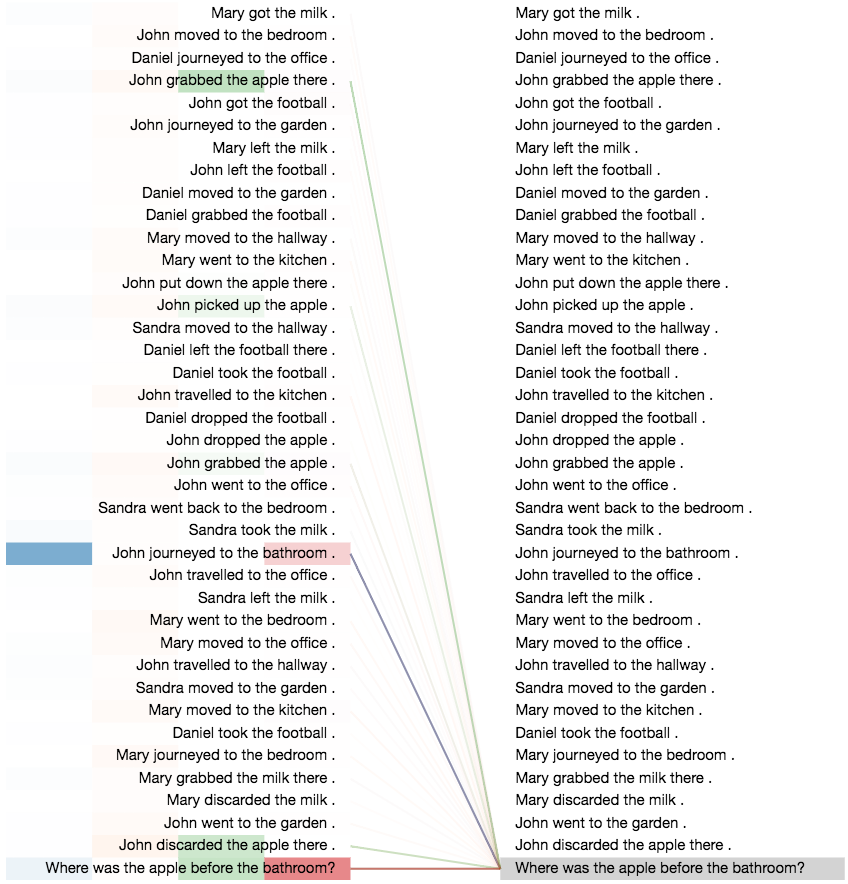
\includegraphics[height=4.2in]{04-part-03/chapter-06/figs_and_tables/figs_attention_babi/e4-step1}
        \caption{Step 1}
    \end{subfigure}%
    \hfill \hfill
    \begin{subfigure}[t]{\textwidth}
        \centering
        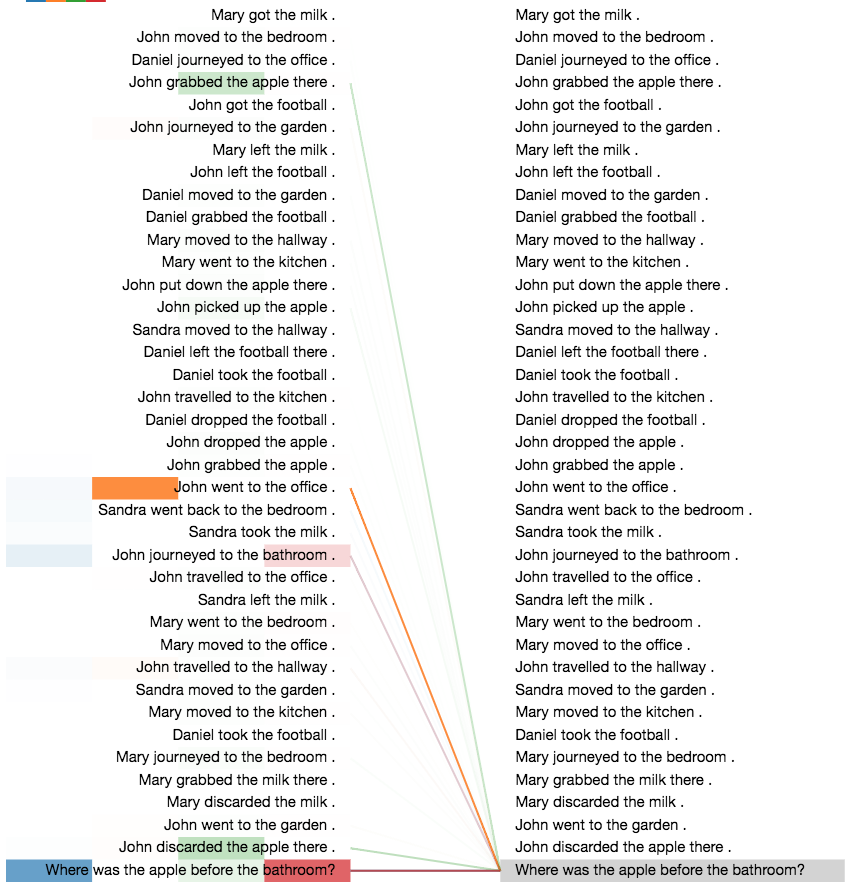
\includegraphics[height=4.2in, trim={0 0 0 0.1cm},clip]{04-part-03/chapter-06/figs_and_tables/figs_attention_babi/e4-step2}
        \caption{Step 2}
    \end{subfigure}
\end{minipage}
\end{figure}
\begin{figure}[h!]\ContinuedFloat
\begin{minipage}{\textwidth}\ContinuedFloat
    \begin{subfigure}[t]{\textwidth}
        \centering
        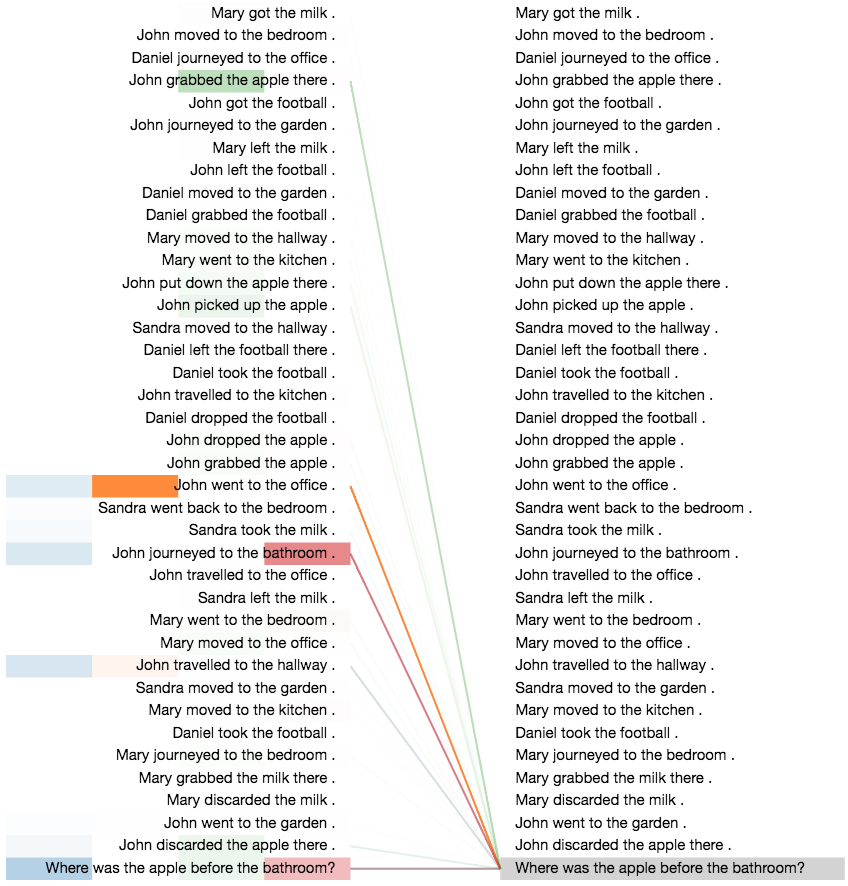
\includegraphics[height=4.2in]{04-part-03/chapter-06/figs_and_tables/figs_attention_babi/e4-step3}
        \caption{Step 3}
    \end{subfigure}
    \hfill \hfill 
    \begin{subfigure}[t]{\textwidth}
        \centering
        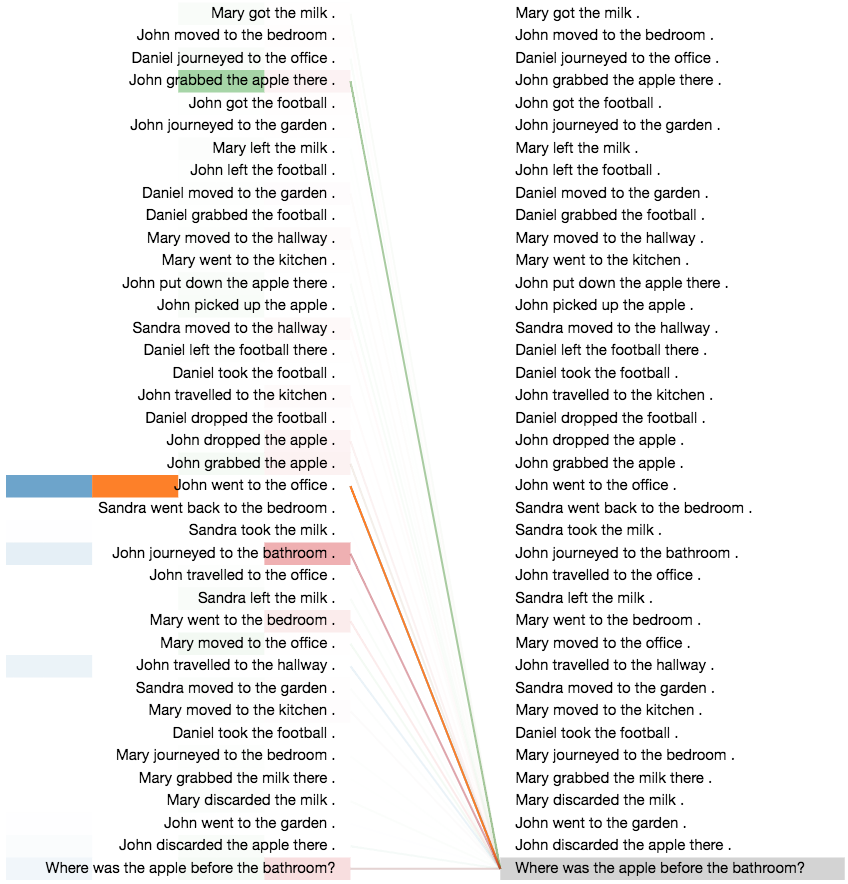
\includegraphics[height=4.2in]{04-part-03/chapter-06/figs_and_tables/figs_attention_babi/e4-step4}
        \caption{Step 4}
    \end{subfigure}
    \caption{\label{fig:ex4}Visualization of the attention distributions, when encoding the question: \emph{``Where was the apple before the bathroom?''}.}
\end{minipage}
\end{figure}

Figures~\ref{fig:ex1}, \ref{fig:ex2}, \ref{fig:ex3}, and \ref{fig:ex4} present visualizations of the attention distributions on bAbI tasks for some examples from Task 1, 2, and 3. The visualization of attention weights is over different time steps based on different heads over all the facts in the story and a question. Different color bars on the left side indicate attention weights based on different heads (4 heads in total).

The above examples illustrate that there is a notion of temporal states in UT, where the model updates its states (memory) in each step based on the output of previous steps, and this chain of updates can also be viewed as steps in a multi-hop reasoning process.

\subsection{Algorithmic Tasks}
The generic neural network architectures cannot generalize well in algorithmic and numerical tasks requiring arithmetic operations such as addition, multiplication etc., even when they may successfully fit any given training data in such tasks, and sometimes they cannot even achieve that~\citep{trask2018neural}. This can be even harder when the distribution of examples' length is different in train and test set.

We trained UTs on three algorithmic tasks, namely Copy, Reverse, and (integer) Addition, all on strings composed of decimal symbols (`0'-`9'). In all the experiments, we train the models on sequences of length 40 and evaluated on sequences of length 400~\citep{neural_gpu} to assess the ability of the models on length generalization.

As an additional inductive bias for UTs on this tasks, when calculating the positional embedding, we use  positions starting with randomized offsets per example. This way, we further encourage the model to learn position-relative transformations, which improves length generalization.
Results are shown in Table~\ref{tab:algorithmic}. Both UT and UT with randomized position offset outperform LSTM and vanilla Transformer by a wide margin on all three tasks. 
The Neural GPU reports perfect results on this task~\citep{neural_gpu}, however we note that this result required a special curriculum-based training protocol which was not used for other models.

\begin{table}[t!]
\centering
    \caption{Accuracy (higher better) on the algorithmic tasks. $^*$Note that the Neural GPU was trained with a special curriculum to obtain the perfect result, while other models are trained without any curriculum.}
    \label{tab:algorithmic}
    \begin{adjustbox}{max width=\textwidth}
    \begin{tabular}{lcccccc}
        & & & & & & \\ \toprule
        \multirow{2}{*}{ \bf Model } & \multicolumn{2}{c}{ \textbf{Copy} } & \multicolumn{2}{c}{ \textbf{Reverse} } & \multicolumn{2}{c}{ \textbf{Addition} } \\ \cmidrule(l{2pt}r{2pt}){2-3} \cmidrule(l{2pt}r{2pt}){4-5} \cmidrule(l{2pt}r{2pt}){6-7}
        & \textit{char-acc} & \textit{seq-acc} & \textit{char-acc} & \textit{seq-acc} & \textit{char-acc} & \textit{seq-acc} \\ \midrule
        \bf LSTM & 0.45 & 0.09 & 0.66 & 0.11 & 0.08 & 0.0 \\
        \bf Transformer & 0.53 & 0.03 & 0.13 & 0.06 & 0.07 & 0.0 \\
        \bf Universal Transformer & 0.76 & 0.29 & 0.83 & 0.41 & 0.32 & 0.02 \\
        \bf UT w/ randomized offset & 0.91 & 0.35 & 0.96 & 0.46 & 0.34 & 0.02 \\
        \bf Neural GPU$^*$ & \textbf{1.00} & \textbf{1.00} & \textbf{1.00} & \textbf{1.00} & \textbf{1.00} &
        \textbf{1.00} \\ \bottomrule
    \end{tabular}
    \end{adjustbox}
\end{table}

\subsection{Learning to Execute (LTE)}
As another class of sequence-to-sequence learning problems, we also evaluate UTs on Learning to Execute (LTE) tasks. 
LTE is a set of tasks indicating the ability of a model to learn to execute computer programs and was proposed by~\citet{ZS14}. These tasks include two subsets: 1) program evaluation tasks (program, control, and addition) that are designed to assess the ability of models for understanding numerical operations, if-statements, variable assignments, the compositionality of operations, and more, as well as 2) memorization tasks (copy, double, and reverse). 

The difficulty of the program evaluation tasks is parameterized by their \textit{length} and \textit{nesting}. The
length parameter is the number of digits in the integers that appear in the programs (so the integers are chosen uniformly from [1, \emph{length}]), and the nesting parameter is the number of times we are allowed to combine the operations with each
other. Higher values of nesting yield programs with deeper parse trees.
For instance, here is a program that is generated with length = 4 and
nesting = 3. 
\begin{table}[h!]
\fontsize{8}{8}\fontfamily{pcr}\selectfont
\begin{tabular}{l l}
\textbf{Input}: & \\
& j=8584 \\
& {\color{blue}{for}} x {\color{blue}{in}} range(8): \\
& ~~j+=920 \\
& b=(1500+j) \\
& {\color{blue}{print}}((b+7567)) \\
\textbf{Target}: & \\
& 25011
\end{tabular}
\end{table}

\begin{table}[t!]
    \centering
    \caption{Character-level (\emph{char-acc}) and sequence-level accuracy (\emph{seq-acc}) results on the Memorization LTE tasks, with maximum length of 55.}
    \label{tab:lte-mem}
    \begin{adjustbox}{max width=\textwidth}
    \begin{tabular}{lcccccc}
        \toprule
        %& \multicolumn{7}{c}{Memorization Tasks} \\
        & \multicolumn{2}{c}{ \bf Copy } & \multicolumn{2}{c}{ \bf Double } & \multicolumn{2}{c}{ \bf Reverse } \\
        \cmidrule(l{2pt}r{2pt}){2-3} \cmidrule(l{2pt}r{2pt}){4-5} \cmidrule(l{2pt}r{2pt}){6-7}
        \bf Model & \textit{char-acc} & \textit{seq-acc} & \textit{char-acc} & \textit{seq-acc} & \textit{char-acc} & \textit{seq-acc} \\ \midrule
        \bf LSTM & 0.78 & 0.11 & 0.51 & 0.05 & 0.91 & 0.32 \\
        \bf Transformer & 0.98 & 0.63 & 0.94 & 0.55 & 0.81 & 0.26 \\
        \bf Universal Transformer & \textbf{1.00} & \textbf{1.00} & \textbf{1.00} & \textbf{1.00} & \textbf{1.00} & \textbf{1.00} \\ \bottomrule
    \end{tabular}
    \end{adjustbox}
\end{table}

\begin{table}[t!]
    \centering
    \caption{Character-level (\emph{char-acc}) and sequence-level accuracy (\emph{seq-acc}) results on the Program Evaluation LTE tasks with maximum nesting of 2 and length of 5.}
    \label{tab:lte-prog}
    \begin{adjustbox}{max width=\textwidth}
    \begin{tabular}{lcccccc}
    \toprule
        & \multicolumn{2}{c}{ \bf Program } & \multicolumn{2}{c}{ \bf Control } & \multicolumn{2}{c}{ \bf Addition } \\ \cmidrule(l{2pt}r{2pt}){2-3} \cmidrule(l{2pt}r{2pt}){4-5} \cmidrule(l{2pt}r{2pt}){6-7}
        \bf Model & \textit{char-acc} & \textit{seq-acc} & \textit{char-acc} & \textit{seq-acc} & \textit{char-acc} & \textit{seq-acc} \\ \midrule
        \bf LSTM & 0.53 & 0.12 & 0.68 & 0.21 & 0.83 & 0.11 \\
        \bf Transformer & 0.71 & 0.29 & 0.93 & 0.66 & \textbf{1.00} & \textbf{1.00} \\
        \bf Universal Transformer & \textbf{0.89} & \textbf{0.63} & \textbf{1.00} & \textbf{1.00} & \textbf{1.00} & \textbf{1.00} \\
    \bottomrule
    \end{tabular}
    \end{adjustbox}
\end{table}

We use the mix-strategy discussed in~\citep{ZS14} to generate the datasets. Unlike~\citep{ZS14}, we do not use any curriculum learning strategy during training and we make no use of target sequences at test time. Tables~\ref{tab:lte-mem} and \ref{tab:lte-prog} present the performance of an LSTM model, Transformer, and Universal Transformer on the program evaluation and memorization tasks, respectively. UT achieves perfect scores in all the memorization tasks and also outperforms both LSTMs and Transformers in all program evaluation tasks by a wide margin. 



\subsection{Subject-Verb Agreement}
Next, we consider the task of predicting number-agreement between subjects and verbs in English sentences~\citep{linzen2016assessing}. Succeeding in this task is a strong indicator that a model can learn to approximate syntactic structure and therefore it was proposed by~\citet{linzen2016assessing} as proxy for assessing the ability of different models to capture hierarchical structure in natural language. 

Two experimental setups were proposed by ~\citet{linzen2016assessing} for training a model on this task: 1) training with a language modeling objective, i.e., next word prediction, and 2) as binary classification, i.e. predicting the number of the verb given the sentence. 
We follow the experimental protocol of ~\citet{linzen2016assessing} for solving the task using a language modeling training setup, i.e.\ a next word prediction objective, followed by calculating the ranking accuracy of the target verb at test time. 

In this task, in order to have different levels of difficulty, ``agreement attractors'' are used, i.e.\ one or more intervening nouns with the opposite number from the subject with the goal of confusing the model. In this case, the model needs to correctly identify the head of the syntactic subject that corresponds to a given verb and ignore the intervening attractors in order to predict the correct form of that verb.
Here are some examples for this task in which subjects and the corresponding verbs are in boldface and agreement attractors are underlined:
\begin{table}[h!]
\fontsize{9}{10}\fontfamily{pcr}\selectfont
\begin{tabular}{l l}
\textbf{No attractor:} & The \textbf{boy} \textbf{smiles}. \\
\textbf{One attractor:}  &  The \textbf{number} of \underline{men} \textbf{is} not clear. \\
\textbf{Two attractors:}  &  The \textbf{ratio} of \underline{men} to \underline{women} \textbf{is} not clear. \\
\textbf{Three attractors:} &  The \textbf{ratio} of \underline{men} to \underline{women} and \underline{children} \textbf{is} not clear. 
\end{tabular}
\end{table}

\begin{table}
\centering
\begin{adjustbox}{max width=\textwidth}
\begin{tabular}{lccccccc}
\toprule
\multirow{2}{*}{ \bf Model } & \multicolumn{6}{c}{ \bf Number of attractors } & \\ \cmidrule{2-7}
& \textit{0} & \textit{1} & \textit{2} & \textit{3} & \textit{4} & \textit{5} & \textit{Total} \\ \midrule
\multicolumn{8}{c}{ \bf Previous best results~\citep{yogatama2018memory}: } \\ \midrule
\bf Best Stack-RNN & \emph{0.994} & 0.979 & 0.965 & 0.935 & 0.916 & 0.880 & 0.992 \\
\bf Best LSTM & 0.993 & 0.972 & 0.950 & 0.922 & 0.900 & 0.842 & 0.991 \\
\bf Best Attention & \textbf{0.994} & \textbf{0.977} & 0.959 & 0.929 & 0.907 & 0.842 & \textbf{0.992} \\ \midrule
\multicolumn{8}{c}{ \bf Our results: } \\ \midrule
\bf Transformer & 0.973 & 0.941 & 0.932 & 0.917 & 0.901 & 0.883 & 0.962 \\
\bf Universal Transformer & 0.993 & 0.971 & \textbf{0.969} & 0.940 & 0.921 & 0.892 & \textbf{0.992} \\
\bf UT w/ ACT & \textbf{0.994}	& 0.969	& 0.967	& \textbf{0.944}	& \textbf{0.932}	& \textbf{0.907}	& \textbf{0.992} \\
\midrule
\bf $\Delta$ (UT w/ ACT - Best) & 0 & -0.008 & 0.002 & 0.009 & 0.016 & 0.027 & - \\
 \bottomrule
\end{tabular}
\end{adjustbox}
\caption{Accuracy on the subject-verb agreement number prediction task (higher is better).}
\label{tab:sva}
\end{table}
Our results are summarized in Table~\ref{tab:sva}. The best LSTM with attention from the literature achieves 99.18\% on this task~\citep{yogatama2018memory}, outperforming a vanilla Transformer~\citep{tran18}. UTs significantly outperform standard Transformers, and achieve an \emph{average} result comparable to the current state of the art (99.2\%). However, we see that UTs (and particularly with dynamic halting) perform progressively better than all other models as the number of attractors increases (see the last row, $\Delta$).


\todo{why ut helps here?}


\subsection{LAMBADA Language Modeling}
The LAMBADA task~\citep{paperno2016lambada} is a language modeling task consisting of predicting a missing target word given a broader context of 4-5 preceding sentences. The dataset was specifically designed so that humans are able to accurately predict the target word when shown the full context, but not when only shown the target sentence in which it appears. It therefore goes beyond language modeling, and tests the ability of a model to incorporate broader discourse and longer term context when predicting the target word\footnote{\url{http://clic.cimec.unitn.it/lambada/appendix_onefile.pdf}}.
Here is a sample from the dataset:

\begin{table}[h!]
\fontsize{8}{10}\fontfamily{pcr}\selectfont
\begin{tabular}{l l}
\textbf{Context}: & \\
& ``Yes, I thought I was going to lose the baby.'' \\
&  ``I was scared too,'' he stated, sincerity flooding his eyes. \\ 
&  ``You were?'' ``Yes, of course. Why do you even ask?''  \\
&  ``This baby wasn't exactly planned for.''
\\
\textbf{Target sentence}: & \\
& ``Do you honestly think that I would want you to have a \_\_\_\_\_\_\_\_?'' 
\\
\textbf{Target word}:  & \\  
& miscarriage
\end{tabular}
\end{table}

The LAMBADA task consists in predicting the target word given the whole passage (i.e., the context plus the target sentence). A ``control set''  is also provided which was constructed by randomly sampling passages of the same shape and size as the ones used to build LAMBADA, but without filtering them in any way. The control set is used to evaluate the models at standard language modeling before testing on the LAMBADA task, and therefore to ensure that low performance on the latter cannot be attributed simply to poor language modeling.

The task is evaluated in two settings: as \emph{language modeling} (the standard setup) and as \emph{reading comprehension}. In the former (more challenging) case, a model is simply trained for next-word prediction on the training data, and evaluated on the target words at test time (i.e.\ the model is trained to predict all words, not specifically challenging target words).  In the latter setting, introduced by Chu et al.~\cite{chu2017broad}, the target sentence (minus the last word) is used as query for selecting the target word from the context sentences. Note that the target word appears in the context 81\% of the time, making this setup much simpler. However the task is impossible in the remaining 19\% of the cases.

\begin{table}[t!]
\centering
    \begin{adjustbox}{max width=\textwidth}
    \begin{tabular}{lcccccc}
    \toprule
    \multirow{2}{*}{ \bf Model } & \multicolumn{3}{c}{\bf LM Perplexity \& (Accuracy) } & \multicolumn{3}{c}{\bf RC Accuracy } \\ \cmidrule(l{2pt}r{2pt}){2-4} \cmidrule(l{2pt}r{2pt}){5-7}
    & \textit{control} & \textit{dev} & \textit{test} & \textit{control} & \textit{dev} & \textit{test} \\ \midrule
    \bf Neural Cache~\citep{grave2016improving} & {\bf 129} & 139 & - & - & - & - \\ 
    \bf Dhingra et al.~\cite{dhingra2018neural} & - & - & - & - & - & 0.5569 \\ \midrule
    \bf Transformer & 142 (0.19) & 5122 (0.0) & 7321 (0.0) & 
    0.4102 & 0.4401 & 0.3988 \\
    \bf LSTM & 138 (0.23) & 4966 (0.0) & 5174 (0.0) & 0.1103 & 0.2316 & 0.2007 \\
    \bf UT \emph{base}, 6 steps (fixed) & 131 (0.32) & 279 (0.18) & 319 (0.17) & {\bf 0.4801} & 0.5422 & 0.5216 \\
    \bf UT w/ dynamic halting & 130 (0.32) & {\bf 134} (0.22) & {\bf 142} (0.19) & 0.4603 & {\bf 0.5831} & {\bf 0.5625} \\ \midrule
    \bf UT \emph{base}, 8 steps (fixed) & 129(0.32) & 192 (0.21) & 202 (0.18) & - & - & - \\
    \bf UT \emph{base}, 9 steps (fixed) & \textbf{129(0.33)} & 214 (0.21) & 239 (0.17) & - & - & - \\
 \bottomrule
    \end{tabular}
    \end{adjustbox}
    \caption{LAMBADA language modeling (LM) perplexity (lower better) with accuracy in parentheses (higher better), and Reading Comprehension (RC) accuracy results (higher better). `-' indicates no reported results in that setting.}
    \label{tab:lambada}
\end{table}

The results are shown in Table~\ref{tab:lambada}. Universal Transformer achieves state-of-the-art results in both the language modeling and reading comprehension setup, outperforming both LSTMs and vanilla Transformers. Note that achieving good results on the control set only shows a model's strength in standard language modeling.

Our best fixed UT results used 6 steps. However, the average number of steps that the best UT with dynamic halting took on the test data over all positions and examples was $8.2 \rpm 2.1$. In order to see if the dynamic model did better simply because it took more steps, we trained two fixed UT models with 8 and 9 steps respectively (see last two rows). Interestingly, these two models achieve better results compared to the model with 6 steps, but \emph{do not outperform the UT with dynamic halting}. This leads us to believe that dynamic halting may act as a useful regularizer for the model via incentivizing a smaller numbers of steps for some of the input symbols, while allowing more computation for others.

\subsection{Machine Translation}
We trained a UT on the WMT 2014 English-German translation task using the same setup as reported in \citep{transformer} in order to evaluate its performance on a large-scale sequence-to-sequence task. Results are summarized in Table~\ref{tab:wmt}. The UT with a fully-connected recurrent transition function (instead of separable convolution) and without ACT improves by 0.9 BLEU over a Transformer and 0.5 BLEU over a Weighted Transformer with approximately the same number of parameters \citep{ahmed2017weighted}.

\begin{table}[t!]
    \centering
    \caption{Machine translation results on the WMT14 En-De translation task trained on 8xP100 GPUs in comparable training setups. All \emph{base} results have the same number of parameters.}
    \begin{tabular}{lc}
        \toprule
        \bf{Model} & \bf{BLEU} \\
        \midrule
        \bf Universal Transformer \emph{small} & 26.8 \\
        \bf Transformer \emph{base}~\citep{transformer} & 28.0 \\
        \bf Weighted Transformer \emph{base}~\citep{ahmed2017weighted} & 28.4 \\
       \bf  Universal Transformer \emph{base} & \bf{28.9} \\
        % \midrule
        % Transformer \emph{big}~\citep{transformer} & ??.? \\
        % Universal Transformer \emph{big} & \bf{??.?} \\
        \bottomrule
    \end{tabular}
    \label{tab:wmt}
\end{table}

\subsection{Open Domain Question Answering}
Open-domain question answering aims to satisfy users who are looking for a direct answer to a complex information need. 
This requires querying large open-domain knowledge sources like the Web. 
Inferring the answer to a question given multiple documents that potentially contain the answer, is at the heart of the open-domain question answering task. 
Most open-domain question answering systems described in the literature first retrieve relevant documents or passages, select one or a few of them as the context, and then feed the question and the context to a reading comprehension system to extract the answer~\citep{buck2017ask, chen2017reading, seo2016bidirectional, dhingra2016gated}. 
However, information needed to answer complex questions is not always contained in a single, directly relevant document that is ranked high. In many cases, there is a need to read multiple documents, combine them, and reason over the facts from these documents to be able to give the correct answer to the question.

For example, in Figure~\ref{fig:example}, in order to infer the correct answer to the question: ``\texttt{Who is the Spanish artist, sculptor and draughtsman famous for co-founding the Cubist movement?}'' given the top-ranked document, a reading comprehension system most likely will extract ``\texttt{Georges Braque}'' as the answer, which is not the correct answer. 
In this example, in order to infer the correct answer, one has to go down the ranked list, gather and encode facts, even those that are not immediately relevant to the question, like ``\emph{Malaga is a city in Spain},'' which can be inferred from a document at rank 66, and then in a multi-step reasoning process, infer some new facts, including ``\emph{Picasso was a Spanish artist}'' given documents at ranks~12 and~66, and ``\emph{Picasso, who was a Spanish artist, co-founded the Cubist}'' given the previously inferred fact and the document ranked third. 

\begin{figure}[!t]
 \centering
 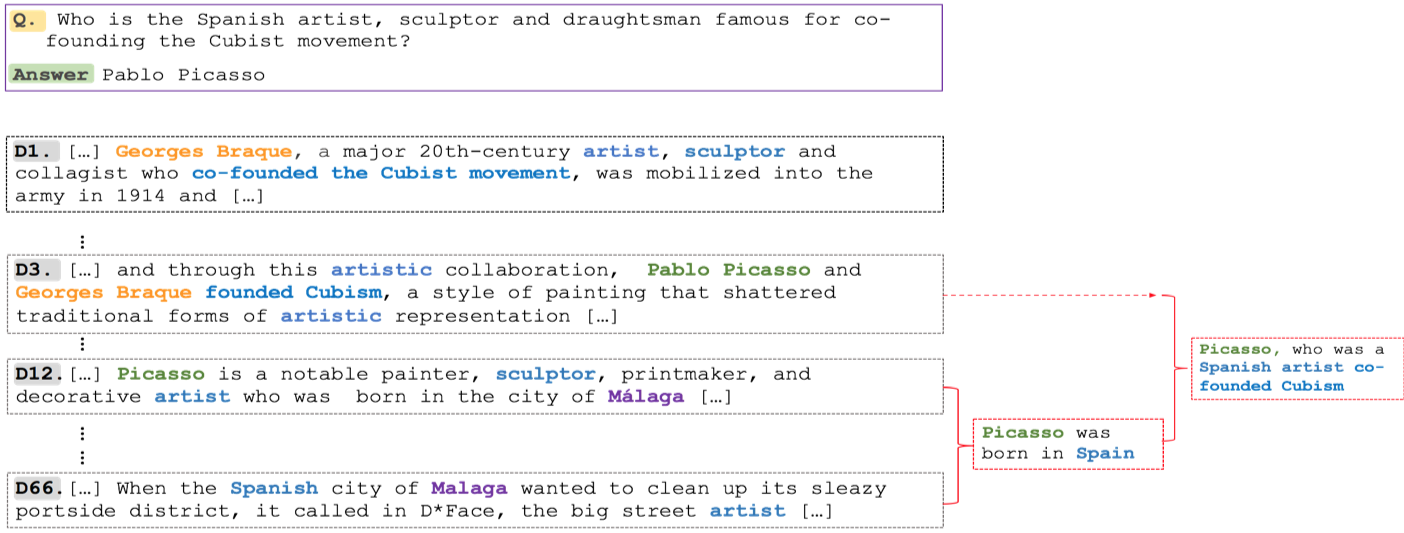
\includegraphics[width=\textwidth]{04-part-03/chapter-06/figs_and_tables/fig_od_example.png}
%  \vspace{1pt}
 \caption{Example complex question answering that requires that information from multiple documents be combined and some amount of reasoning over the information extracted from those documents. (Best viewed in color.)}
 \label{fig:example}
\end{figure}

In this example, and in general in many cases in open-domain question answering, a piece of information in a low-ranked document that is not immediately relevant to the question, may be useful to fill in the blanks and complete information extracted from the top relevant documents and eventually support inferring the correct answer.
However, most open-domain question answering methods focus on only one or a few candidate documents by filtering out the less relevant documents to avoid dealing with noisy information and operate over the selected set of documents to extract the answer~\citep{wang2017r, wang2017evidence,lin2018denoising}. 

We propose a new architecture, called \tracrnet (pronounced \emph{Tracker Net}, that combines Transformer and  Universal Transformer to improve open-domain question answering by explicitly operating on a larger set of candidate documents during the whole question answering process and learning how to aggregate and reason over information from these documents in an effective way while trying not to be distracted by noisy documents. 
% 
Given the candidate documents and the question, to generate the answer, \tracrnet first \underline{\textbf{Tra}}nsforms them into vectors by applying a stack of  Transformer blocks with self-attention over words in each document in a layer called \emph{Input Encoding}. 
Then, it updates the learned representations from the first stage by \underline{\textbf{C}}ombining and enriching them through a multihop \underline{\textbf{R}}easoning process by applying multiple steps of the Universal Transformer in a layer called \emph{Multihop Reasoning}.  

% paragraph might be too verbose
Returning to the example in Figure~\ref{fig:example}, after learning representations for each top-ranked document and the question, \tracrnet updates them by applying multiple steps of the Universal Transformer. 
Given the self-attention mechanism and inductive bias of the Universal Transformer, in the first step, \tracrnet can update the representation of document D\#12 by attending to D\#66 (as they are related by both mentioning Malaga) and augment the information in D\#12 with the fact that ``Malaga is city in Spain,'' so the updated vector of D\#12 has the fact that ``Picasso is a Spanish artist'' encoded in itself. 
Then, in the next step of reasoning, \tracrnet can update the representation of D\#3 by attending over the vector representing D\#12 estimated in the previous step, and enrich the information in D\#3 with the fact that ``Picasso is a Spanish artist,'' and the updated vector of D\#3 has the fact that ``Picasso, who was a Spanish artist co-founded Cubism'' encoded in it. 
After that, during answer generation, the decoder can attend to the final vector representing D\#3 and give the correct answer.

% why \tracrnet rocks:
% 1. fast
\tracrnet has a number of desirable features.
%
First, all the building blocks of \tracrnet are based on self-attentive feed-forward neural networks, hence per-symbol hidden state transformations are fully parallelizable, which leads to an enormous speedup during training and a super fast input encoding during inference time compared to RNN based models. 
% 3. It can reason
Second, while there is no recurrence in time in our model, the recurrence in depth in the Universal Transformer used in the \emph{Multihop Reasoning} layer, adds the inductive bias to the model that is needed to go beyond understanding each document separately and combine their information in multiple steps.
% 2. global receptive field -> long docs, a large set of docs
Third, \tracrnet has the global receptive field of the Transformer based models~\citep{vaswani2017attention,Dehghani:ICLR:2019}, which helps it to better encode a long document during \emph{Input Encoding} as well as perform better inference over a rather large set of documents during \emph{Multihop Reasoning}.
% 4. robustness against noise
And fourth, the hierarchical usage of a self-attention mechanism, first over words and then over documents, helps \tracrnet to control its attention both at word and document levels, making it less fragile to noisy input, which is of key importance while encoding many documents.
%
All these properties of \tracrnet come together and lead to an effective and efficient architecture for open-domain question answering. 

We employ \tracrnet on two public open-domain question answering datasets, SearchQA and Quasar-T, and achieve results that meet or exceed the state-of-the-art. 

\subsubsection{\tracrnet} % : Transform, Combine, and Reason}
\label{sec:tra}
In the setup we consider here, the model is given a question $q$ and a set of $n$ relevant documents $C_q=\{D^q_1, D^q_2, \ldots D^q_n\}$ retrieved from the web using a search engine as the input, and the goal is to ``generate'' the answer $a_q$ to the question $q$ based on the supporting document(s) in the set $C_q$.

This is different from the standard Reading Comprehension (RC) tasks~\cite{hermann2015teaching,xiong2016dynamic}. 
First of all, in RC a single document (passage) is given, from which the answer should be extracted. 
Secondly, in RC a strong supervision on the positions of the answer spans is available during training.
We also assume that the utilized information or techniques to retrieve relevant documents are not available to the model, therefore there is no leverage for getting better-supporting documents.

\begin{figure}[!t]
 \centering
 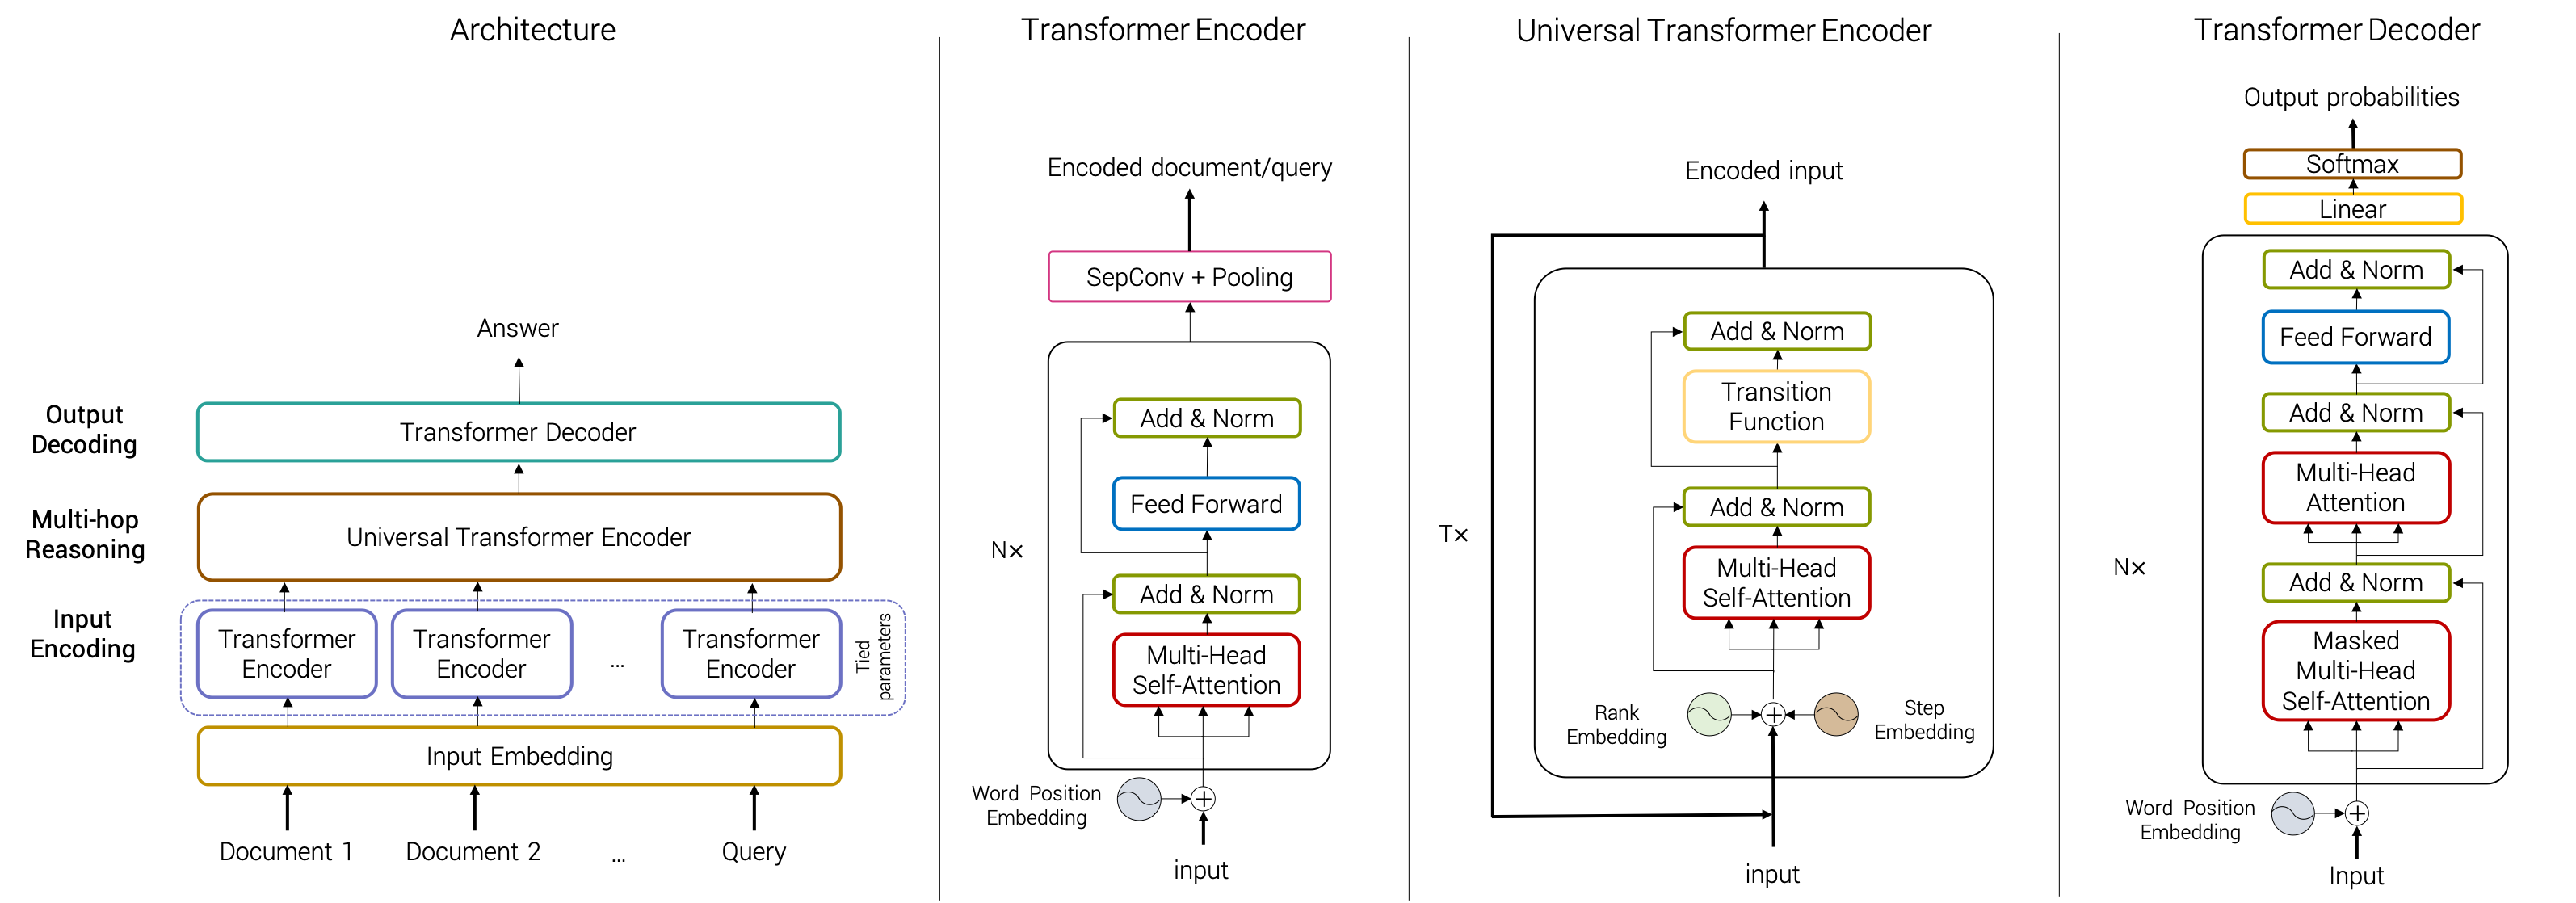
\includegraphics[width=\textwidth]{04-part-03/chapter-06/figs_and_tables/fig_tracrnet.png}
 \caption{An overview of the \tracrnet architecture.}
 \label{fig:model}
\end{figure}

\tracrnet is based on the encoder-decoder architecture, where we have a hierarchy of transformer-based models in the encoder, where the model can attend first over words and then over documents~\citep{Dehghani2017:CIKM}. At the bottom, in the \emph{Input Encoding} layer, we encode each document in $C_q$ as well as the question with transformer blocks with tied parameters that are fed by word-level embeddings. 
Then, we feed the encoded documents and the question from this layer to the \emph{Multihop Reasoning} layer which is, in fact, a universal transformer block where representations of all documents and the question get iteratively updated using multiple steps of self-attention.
Then, we use a stack of transformer decoder blocks as the \emph{Output Decoder} layer to generate the answer. 
%
The general schema of \tracrnet is depicted in Figure~\ref{fig:model}. 
Below, we explain the details of each of these layers in the model.

\mypar{Input encoding} 
The Input Encoding layer is in charge of encoding each of the documents and the question to single vectors given their words' embeddings. For this layer, we used a stack of $N$ Transformer Encoder blocks that is followed by a depth-wise separable convolution~\citep{kaiser2017depthwise,chollet2017xception} and then a pooling function to get a single vector representation for the whole document or the question  (see  the \texttt{Transformer Encoder} in Figure~\ref{fig:model}) . 
Depth-wise separable convolution is defined by a convolution on each of the feature channels separately, followed by a point-wise convolution that is applied to project them to a feature vector with the desirable depth (see \citep{chollet2017xception} for more details).

\mypar{Multihop reasoning} 
Multihop Reasoning is the layer in which the Universal Transformer is employed to combine evidence from all documents with respect to the question within a multi-step process with the capacity of multihop reasoning.
%
In \tracrnet, the input of the Universal Transformer Encoder is the set of vectors each representing a document in $C_q$ or the question, that are computed by the \emph{Input Encoding} layer  (see  the \texttt{Universal Transformer Encoder} in Figure~\ref{fig:model}). 

In each step of the Universal Transformer, given $H_{t} \in \mathbb{R}^{(|C_q|+1) \times d}$ and the dimension $d$ of the input vectors, we add two embeddings to $H^{t}$: a \emph{Rank Embedding} that encodes the rank of documents given by the retrieval system, also used to distinguish the question from documents (similar to the positional embedding in token level inputs) and the \emph{Step Embedding}. We use Equation\ref{eqn:coordinate-embeddings} to calculate these embeddings.
In our experiments, we use depthwise separable convolution~\cite{chollet2017xception} as the Transition($\cdot$) function.

In the multihop reasoning layer, the representations of all the documents and question learned from the previous layer get updated during $T$ steps of iterating over the Universal Transformer Encode block. 
Self-attention in this layer allows the model to understand each of the documents based on the information in all the as well as the question.
In addition, the depth-wise recurrency in the Universal Transformer establishes connections among documents at each step and lays the ground for performing multihop reasoning to solve cases similar to what we have shown in Example~\ref{fig:example}.

\mypar{Output decoder} 
After $T$ steps of refining the representations of documents and the question in the Universal Transformer Encoder, the final output is a matrix of $d$-dimensional vector representations $H \in \mathbb{R}^{(|C_q|+1) \times d}$ for all the documents in $C_q$ and the question $q$.

Given this, we use a stack of $N$ Transformer Decoder blocks (see  the \texttt{Universal Transformer Encoder} in Figure~\ref{fig:model}) to decode the answer.
To generate answer from the model at inference time, we run the model autoregresively~\citep{graves2013generating}, where the model consumes the previously generated symbols at each time step in order to generate the distribution over the vocabulary for the next symbol. From this distribution, we select the symbol with highest probability as the next symbol.   


\subsubsection{Datasets}
We have conducted experiments on two publicly available open-domain question answering datasets: SearchQA~\citep{dunn2017searchqa} and Quasar-T~\citep{dhingra2017quasar}. 
In both of these datasets, candidate documents (passages) for each question have already been retrieved using a search engine and we do not add any extra documents to these result sets. 
On both datasets, the human performance is evaluated in a setup where the human subjects try to find the answers to the given question from the same documents retrieved by the IR model.

\mypar{SearchQA}
SearchQA\footnote{\url{https://github.com/nyu-dl/SearchQA}} is a dataset of 140k question-answer pairs crawled from J!\ Archive, and augmented with text snippets retrieved using the Google search engine. 
For each question-answer pair, on average, about 50 web page snippets have been collected. 
In our experiments, we do not use the additional meta-data in the dataset like the snippet's URL.

\mypar{Quasar-T}
Quasar-T\footnote{\url{https://github.com/bdhingra/quasar}} consists of 43k open-domain trivia questions and their answers obtained from various internet sources. 
The set of candidate documents for each question is retrieved using ``Lucene'' from the ClueWeb09 corpus as the background corpus. 
In this dataset, for each question-answer pair, a set of 100 unique passages were collected as candidate documents.

\subsubsection{Model configuration and experimental setup}
We use WordPiece embeddings~\citep{wu:2016:google} with a $32k$ token vocabulary. 
%
In both \emph{Input Encoder} and \emph{Output Decoder} layers, we use 
a stack of 6 Transformer blocks with hidden\_size $= 512$, num\_attention\_heads $=8$, and batch\_size $=2,048$. 
The rest of the hyper-parameters are set to the default values of the Transformer model.
%
In the \emph{Multihop Reasoning} layer, we have a Universal Transformer Encoder with hidden\_size $=512$ and num\_attention\_heads $=4$. 
We set the number of recurrent steps in depth to 12. The rest of the hyper-parameters are set to the default values of the Universal Transformer model.
%
We train with batch size of $4,096$ tokens. We use Adam with learning rate of $1e-9$, $\beta_1 = 0.9$, $\beta_2 = 0.98$, $L_2$ weight decay of $1e-04$, learning rate warmup over the first $16,000$ steps, and linear decay of the learning rate. 
We use a dropout probability of $0.1$ on all layers.
%
Since in our model answers are generated using the decoder instead of extracting from the context (detecting spam), to improve the quality of generation, we pretrain all the parameters of the Transformer decoder downstream of the task of language modeling. The embeddings are shared between encoder and decoder, thus the \emph{Input Embedding} layer also enjoys the pretraining. This helps to improve the performance especially in terms of metrics that consider the exact match of the generated answer with the ground truth.
%
During the training of the model, we use teacher-forcing, i.e., the decoder input is the gold target, shifted to the right by one position which is the usual setup for training autoregressive models~\citep{williams1989learning}. 

In our experiments, \tracrnet and its variants are trained on 8 P100 GPUs for $800k$ training steps.
%
For both datasets, a prepared version by \citet{wang2017r} is used in our experiments to train and evaluate the \tracrnet as well as all the baselines. As the $C_q$, we consider top-50 top documents for the SearchQA, and top-100 for the Quasar-T.
%
Following previous work on reading comprehension and open-domain question answering~\citep{shen2017reasonet,buck2017ask,wang2017r,wang2017evidence,lin2018denoising} as our evaluation metrics we adopt the F1 score, that loosely measures the average overlap between the predicted answer and the ground truth answer, and Exact Match (EM) that measures the percentage of predictions that match one of the ground truth answers exactly.\footnote{We use the tool from SQuAD~\citep{rajpurkar2016squad} for evaluation.} 

\subsubsection{Results and Discussion}

\mypar{Baselines} 
We compare our results with the best reading comprehension and open-domain question answering models as well as research that achieves state-of-the-art on the SearchQA and Quasar-T datasets. 
To have a true apples-to-apples comparison, we only consider baselines that use no additional resources to solve the task for these datasets. 
We use the following methods as baselines:
\begin{enumerate}[leftmargin=*]
    \item BiDAF~\citep{seo2016bidirectional}, which is a reading comprehension model with bi-di\-rectional attention flow network that uses the concatenation of top-ranked candidate documents as the context.
    \item R$^3$~\citep{wang2017r}, which is a reinforcement learning approach that uses a ranker for selecting the most confident paragraph to train the reading comprehension model.
    \item \citet{wang2017evidence}'s model, which learns to re-rank the answers extracted by applying an R$^3$ model on multiple documents based on coverage and strength of each of the documents given the question.
    \item \citet{lin2018denoising}'s model, which is the most recent paper achieving state-of-the-art performance on the datasets we use for evaluation. 
    They propose to decompose the process into a document selection to filter out noisy paragraphs, and a paragraph reader to extract the correct answer from the filtered documents. 
    Finally, they aggregate multiple answers to obtain the final answer.
\end{enumerate}
%
Table~\ref{tab:main_results} presents the results of the baseline models, \tracrnet, and the human performance on both datasets.

\begin{table}[!t]
    \centering
    \caption{Performance of \tracrnet compared to the baseline models}
    \label{tab:main_results}
    \begin{adjustbox}{max width=0.7\textwidth}
    \begin{tabularx}{\linewidth}{Xccccc}
        \toprule
        \multirow{2}{*}{\textbf{model}} & \multicolumn{2}{c}{\textbf{SearchQA}} & & \multicolumn{2}{c}{\textbf{Quasar-T}}\\
        \cmidrule{2-3}\cmidrule{5-6}
         & \textbf{EM} & \textbf{F1}  & & \textbf{EM} & \textbf{F1} \\
         \midrule
         BiDAF~\citep{seo2016bidirectional}
         &  28.6  & 34.6 & &  25.9 & 28.5\\
         R$^3$~\citep{wang2017r}
         &  49.0 & 55.3 &  & 35.3 & 41.7 \\
         \citet{wang2017evidence} 
         & 57.0 & 63.2 &  & 42.3 & 49.6  \\
         \citet{lin2018denoising} 
         &  \textbf{58.8}  & 64.5 &  & 42.2 & 49.3 \\
         \tracrnet
         & 52.9 & \textbf{65.1} &  & \textbf{43.2} & \textbf{54.0} \\ \midrule
         Human Performance
         & 43.9 & -- &  & 51.5 & 60.6 \\
         \bottomrule
    \end{tabularx}
    \end{adjustbox}
\end{table}


\mypar{Main results} 
\tracrnet outperforms all the baselines and achieves a new state-of-the-art  (to the best of our knowledge) on the Quasar-T dataset and performs as good as the best performing baseline on the SearchQA dataset.
%
The main advantage of \tracrnet over the baselines is that it makes ``full'' use of the information of ``all'' the candidate documents in $C_q$. 
The models proposed by \citet{lin2018denoising} and \citet{wang2017evidence} are the strongest baselines on these datasets. 
Although they try to capture evidence from multiple sources by reranking or aggregating answers extracted from different documents, they filter out documents that are less likely to help at the beginning of the process. 
In this fashion, they lose the chance of using information from documents that are not directly relevant, like documents \#12 or/and \#66 in Example~\ref{fig:example}. 
However, \tracrnet keeps operating on the full set of candidate documents during the whole process and learns to which extent each document contributes to infer the final answer. 

In SearchQA, we notice that for most of the questions, the answer can be extracted given a single document and in many cases, no multi-document multihop reasoning is required. 
Therefore, since \tracrnet \emph{generates} the answer, as opposed to the baseline models that \emph{extract} the answer from context, it gets a lower EM score. However, in terms of F1 score, \tracrnet slightly improves over the best baseline.

\mypar{Effect of multihop reasoning}
In order to investigate the effect of the \emph{Multihop Reasoning} layer, we handicap \tracrnet by removing this layer and evaluate it in two cases:
\begin{enumerate}[leftmargin=*]
    \item \tracrnet{$_\text{no-mhr}^\text{d}$}, in which the decoder has access to document-\:level representations from the encoder, and 
    \item \tracrnet{$_\text{no-mhr}^\text{w}$} where pooling operation is removed and the decoder has access to word-level representations from the encoder.
\end{enumerate}    
Table~\ref{tab:no_mhr_results} presents the results of the model in these situations.

\begin{table}[!t]
    \centering
    \caption{Performance of \tracrnet with and without the \emph{Multihop Reasoning} layer; numbers in parenthesis indicate percentage of performance loss}
    \label{tab:no_mhr_results}
    \begin{adjustbox}{max width=0.7\textwidth}
    \begin{tabularx}{\linewidth}{@{}Xc@{~~}c@{~~}c@{~~}c@{~~}c@{}}
        \toprule
        \multirow{2}{*}{\textbf{model}} & \multicolumn{2}{c}{\textbf{SearchQA}} & & \multicolumn{2}{c}{\textbf{Quasar-T}}\\
        \cmidrule{2-3}\cmidrule{5-6}
         & \textbf{EM}  & \textbf{F1}  & & \textbf{EM} & \textbf{F1} \\
         \midrule
         \tracrnet
         & 52.9 \phantom{($-8\%$)} & 65.1 \phantom{($-8\%$)}&  & 43.2 \phantom{($-16\%$)}& 54.0 \phantom{($-25\%$)} \\
         \tracrnet{$_\text{no-mhr}^\text{d}$} 
         & 48.6 ($-8\%$) & 61.7 ($-5\%$) &  & 36.4 ($-16\%$) &  43.6 ($-19\%$)\\
         \tracrnet{$_\text{no-mhr}^\text{w}$}
         & 50.2 ($-5\%$) & 59.3 ($-9\%$) &  & 38.1 ($-12\%$) &  40.2 ($-25\%$) \\
         \bottomrule
    \end{tabularx}
    \end{adjustbox}
\end{table}

\begin{figure}[!t]
    \centering
    \begin{subfigure}[t]{\textwidth}
        \centering
        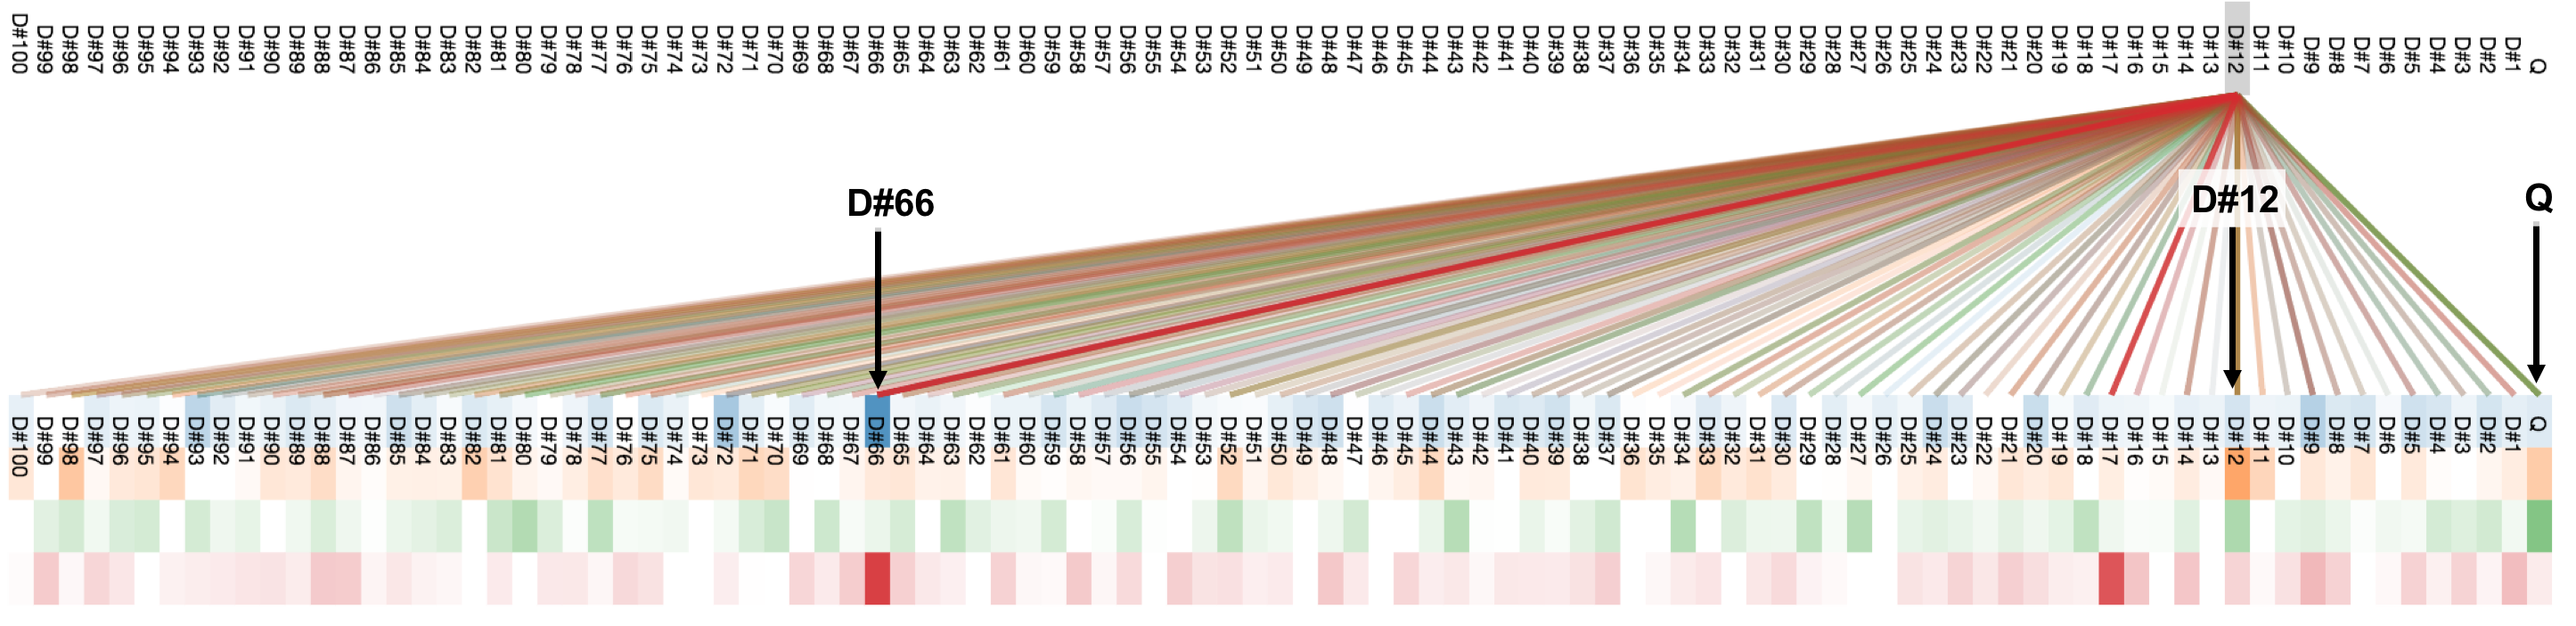
\includegraphics[width=\textwidth]{04-part-03/chapter-06/figs_and_tables/fig_att_tracrnet_step3.png}
        \caption{\label{fig:attention_vis_a}Attention distribution %over different documents and the question 
        when transforming the document at rank 12, in step\#3 of multihop reasoning.}
    \end{subfigure}%
    \vfill
    \begin{subfigure}[t]{\textwidth}
        \centering
        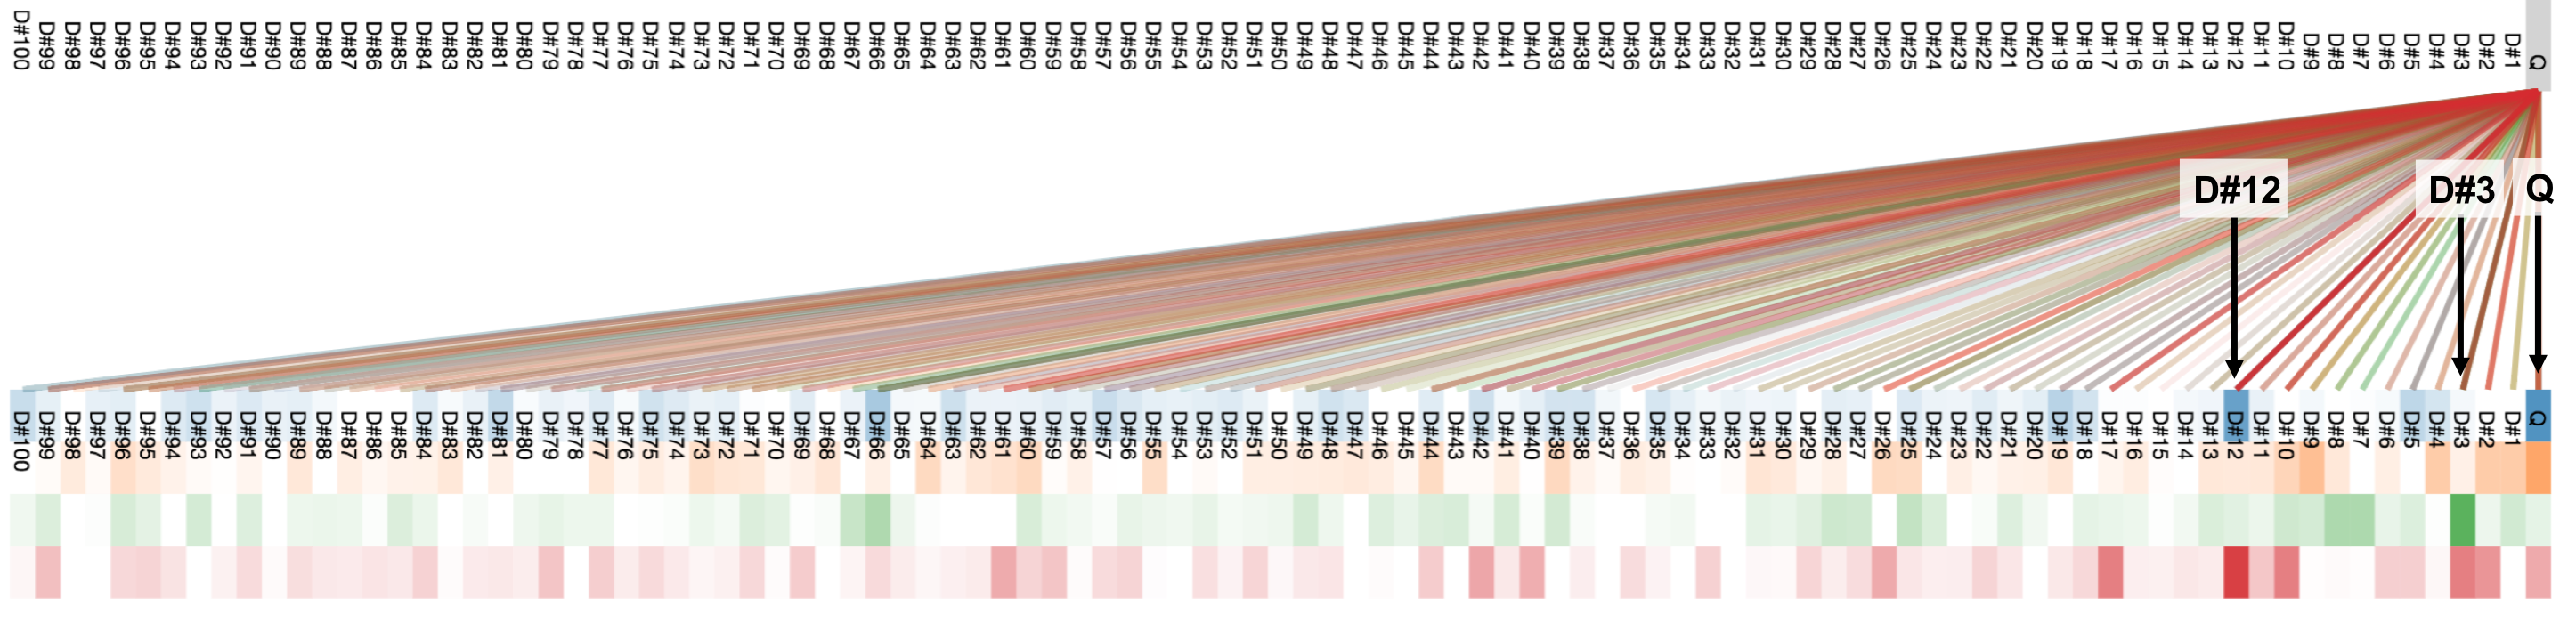
\includegraphics[width=\textwidth]{04-part-03/chapter-06/figs_and_tables/fig_att_tracrnet_step7.png}
        \caption{\label{fig:attention_vis_b}Attention distribution %over different documents and the question 
        when transforming the question, in step\#7 of multihop reasoning.}
    \end{subfigure}
     \caption{Visualization  of multi-head self-attention on Multihop Reasoning layer of \tracrnet. 
     (Best viewed in color.)}
     \label{fig:attention_vis}
\end{figure}

On all measures and datasets, the performance drops when we remove the \emph{Multihop Reasoning} layer. 
The drop in the performance is larger on the Quasar-T dataset than on the SearchQA dataset.
We noticed that trivia questions in Quasar-T, in many cases, contain clauses that should be considered together with and/or operations to be able to give the correct answer. 
For instance, to answer the question ``What Australian food was discovered by John McAdam,'' we should consider that ``the food is Australian'' \emph{and} ``the food is discovered by John McAdam.'' 
In this situation, the chance of having multiple documents each containing one of these facts increases. 
Thus, having multiple supporting documents and the need for reasoning (similar to Example~\ref{fig:example}) will be the exact point where the advantage of the \emph{Multihop Reasoning} layer kicks in.

Another observation here is that when we remove the \emph{Multihop Reasoning} layer, passing word-level embeddings from the encoder to the decoder leads to better EM scores, but not to improved F1 scores. 
The main reason is that, in this situation, access to the input words from the decoder is more explicit. 
This helps the model to get closer to answer extraction than pure answer generation.

For the test example that is presented in Figure~\ref{fig:example}, we observed that all baseline models output ``Georges Braque'' which is extracted from the document at rank~1. 
However, unlike all the baselines, \tracrnet returns the correct answer. 
We looked into the attention distributions in the \emph{Multihop Reasoning} layer of \tracrnet at different steps (of the employed Universal Transformer with 12 depth-wise recurrent steps). 
We were able to find a relation between attention distributions and the reasoning steps that are needed to give the correct answer to this question. 
We illustrate this in Figure~\ref{fig:attention_vis}.

Figure~\ref{fig:attention_vis_a} presents the attention distribution over all documents and the question while encoding the document at rank~12 at step~3. 
\tracrnet has a high level of attention for the document at rank~66 using heads~1 and~4 (blue and red) as well as for the question using head~3 (green) while transforming the document at rank~12. 
This is in accordance with the fact that the model first needs to update the information encoded in the document at rank 12 with the fact that ``Malaga is a city in Spain'' from the document at rank~66. 
Later, at step~7, while encoding the question (Figure~\ref{fig:attention_vis_b}), \tracrnet attends over document 12, which has information about ``Picasso who is a Spanish artist'' (updated in step~3) using heads~1 and~4 and document~3, which contains information about ``Picasso as a co-founder of Cubism'' using head~2 (green). 

\subsubsection{Impact of the number of documents}
As we explained before, unlike most of the previous work that filters candidate documents and narrows down the set of documents under consideration to either a single document or a small set of highly relevant documents before applying an answer extractor to them, \tracrnet uses the full set of candidate documents retrieved by the search engine during the entire process of generating the answer. 
This is of great advantage as our analysis shows that, for some questions, the correct answer can only be extracted when considering information from low-ranked documents that are not immediately relevant to the question.
However, this can potentially come at the cost of (1)~efficiency, as we need to process a larger input, and of (2)~performance, as there will be more noisy and non-relevant documents when we go down the ranked list of candidate documents. 
%
Making use of self-attentive feed-forward neural networks as building blocks of \tracrnet brings the ability of full per-symbol parallelization and leads to an enormous speedup on encoding the input documents. This lets the model encode a larger set of candidate documents efficiently. 

\begin{figure}[!t]
 \centering
 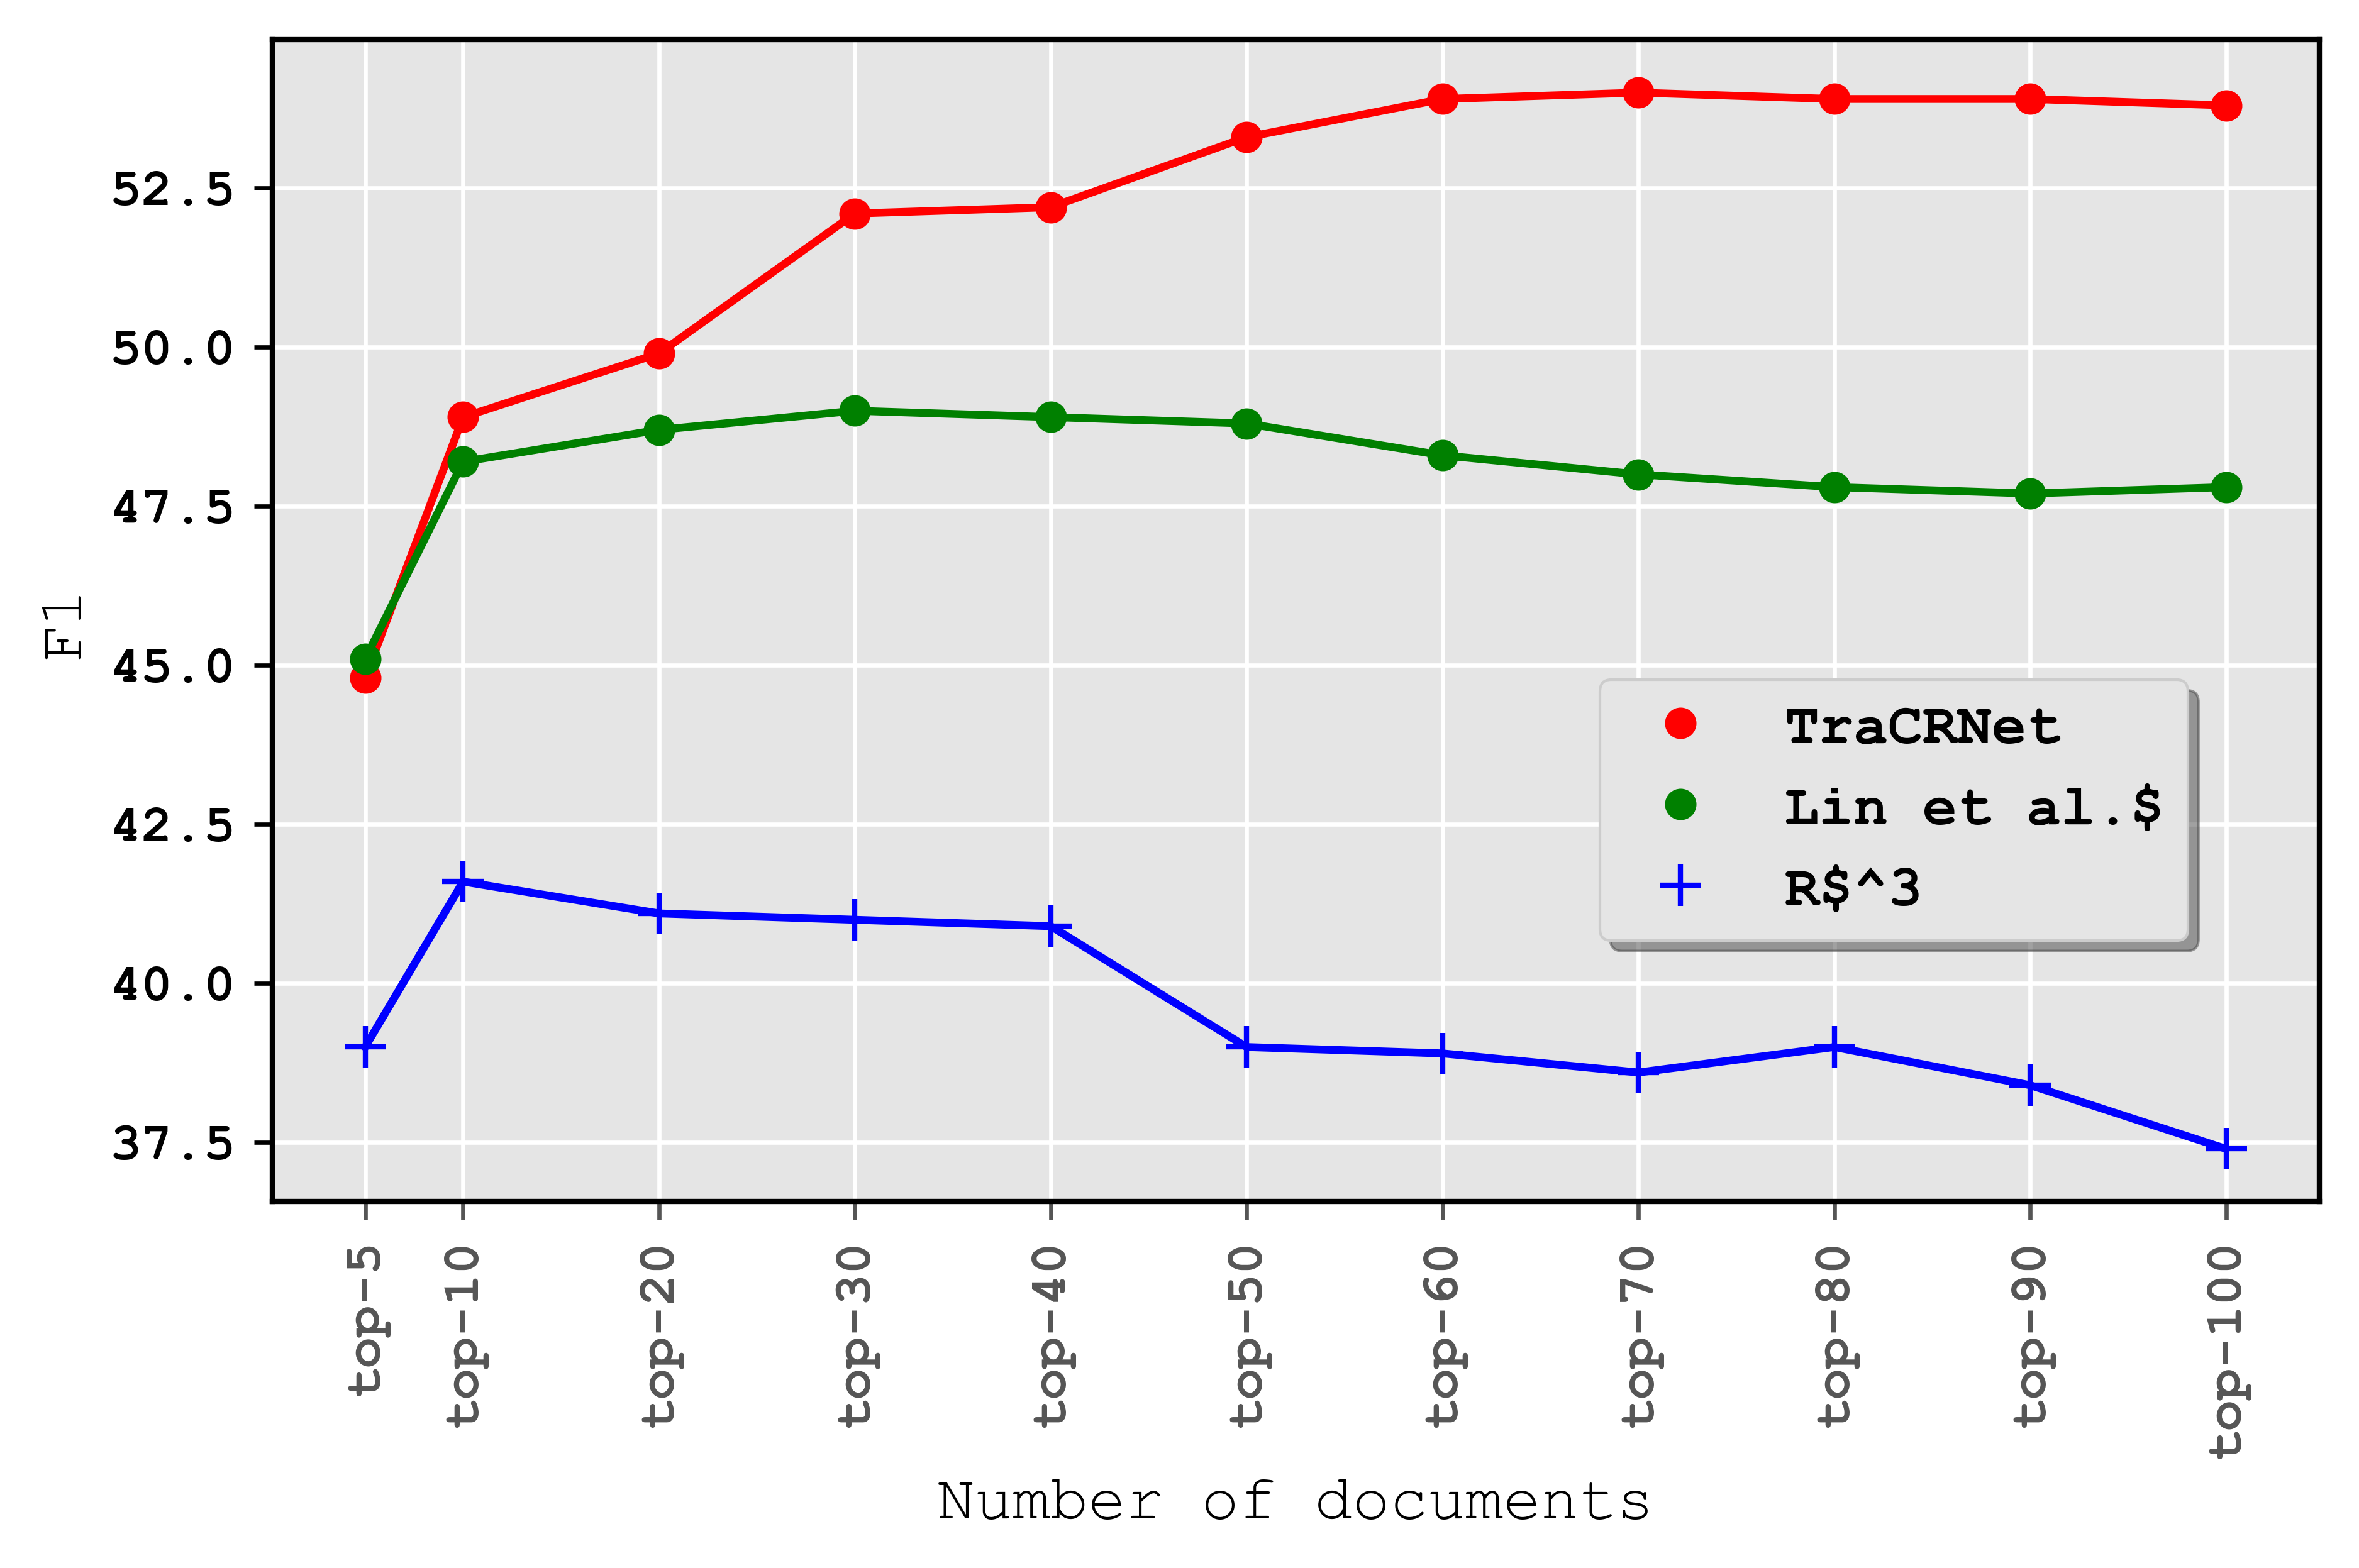
\includegraphics[width=0.6\textwidth]{04-part-03/chapter-06/figs_and_tables/plot_different_num_docs.png}
  %\vspace{5pt}
 \caption{Performance in terms of F1 of \tracrnet and baselines (R$^3$~\citep{wang2017r} and \citet{lin2018denoising}'s model) with different numbers of candidate documents on Quasar-T dataset.}
 \label{fig:diff_num_docs}
\end{figure}

To study how the performance of \tracrnet is affected by the number of candidate documents, we train and evaluate \tracrnet as well as R$^3$~\citep{wang2017r} and \citet{lin2018denoising}'s model on the Quasar-T dataset, using different numbers of candidate documents associated with each question.\footnote{In this experiment, we just change the initial number of candidates, but we train baseline models with their original setups and do not impose any assumption (e.g., fixing the candidate list) on them.}
%
Figure~\ref{fig:diff_num_docs} presents the performance of these models when they are fed with the top-5, top-10, \ldots, top-100 retrieved documents. 
%
As can be seen, although \citet{lin2018denoising}'s model is pretty good at staying robust when noise increases (it is designed to learn from distant supervision), increasing the number of candidate documents eventually leads to a small drop in performance of both baselines due to the noise in the low-ranked documents. 
However, \tracrnet not only controls the effect of noisy low-ranked documents by calibrating their effect on inferring the final answer through self-attention, but it also keeps improving as we increase the number of documents as it can exploit any useful information contained in low-ranked documents which can help better understand the question or perform reasoning.



